\chapter{Implementation}

This chapter details the practical implementation of the BK-MInD system architecture. The chapter is organized as follows: Section~\ref{sec:impl_evolution} describes the evolution from the Phase~1 prototype to the Phase~2 production system. Section~\ref{sec:impl_pipeline} covers the complete Data Processing Pipeline. Subsequent sections address chunking and embedding strategies, indexing and storage, asynchronous job handling, content safety, database schemas, core API services, system deployment, and security implementation details.

\section{Implementation Evolution}\label{sec:impl_evolution}

The development of the Unified MRAG system was executed in two distinct phases, representing a transition from a research-oriented baseline to a robust, production-ready platform. This evolution was driven by the need for scalability, and high availability.

Phase 1 focused on the validation of the core retrieval-augmented generation logic, utilizing local resources and monolithic processing scripts. Phase 2 involved a comprehensive refactoring of the system into a cloud-native architecture, offloading compute-heavy tasks and leveraging managed services for data persistence and orchestration.

\subsection{Phase 1: Foundation and Feasibility}

Phase 1 was characterized by the development of a \textbf{Proof-of-Concept (PoC)} baseline. The primary objective was to validate the technical feasibility of the multimodal retrieval logic and ensure that the integration of text and visual embedding models yielded coherent results. During this stage, the system was implemented as a monolithic Python environment, relying on local filesystem storage for documents and a local instance of a Vector Database for retrieval. While functional, this architecture suffered from significant limitations:

\begin{itemize}
    \item \textbf{Resource Contention}: Running heavy embedding models (like ColQwen) alongside the API server on a single machine led to significant latency and memory exhaustion.
    \item \textbf{Lack of Persistence}: User sessions and processing states were transient, meaning that any system restart resulted in the loss of progress and required complete re-indexing of documents.
    \item \textbf{Monolithic Bottlenecks}: The sequential nature of the data processing pipeline meant that large document uploads blocked all other system operations, preventing concurrent usage.
\end{itemize}

\subsection{Phase 2: Scalability and Productionalization}

Phase 2 involved a fundamental \textbf{architectural refactoring}, transitioning the system into a production-grade, cloud-native application. The focus shifted from functional correctness to operational excellence, addressing the bottlenecks identified during Phase 1. Key enhancements included:

\begin{itemize}
    \item \textbf{Decoupled Infrastructure}: The core compute logic was separated from the storage and inference layers. By leveraging \textbf{Amazon S3} for object storage and \textbf{Qdrant Cloud} for vector search, the system achieved true multi-tenancy and horizontal scalability.
    \item \textbf{Stateful Session Management}: The integration of \textbf{Amazon DynamoDB} allowed for persistent, low-latency tracking of user chat histories and processing statuses, enabling a seamless resume-from-anywhere experience.
    \item \textbf{Optimized Inference Offloading}: To handle the massive compute requirements of late-interaction models, Phase 2 offloaded visual embedding generation to \textbf{AWS SageMaker} using GPU-accelerated inference endpoints (ml.g4dn.xlarge instances with single NVIDIA T4 GPU, 4 vCPU, 16GB RAM). This configuration provides approximately 250-300 embeddings/second throughput for ColQwen inference, ensuring that the main application backend remains responsive even during high-intensity batch processing of document pages. SageMaker auto-scaling adjusts instance counts from 1 to 5 based on endpoint invocation load, balancing cost-efficiency during off-peak hours with throughput during peak usage.
    \item \textbf{Asynchronous 7-Stage Pipeline}: The processing logic was rebuilt as a concurrent, event-driven pipeline with intelligent conditional routing. Stages 3b, 3c, and 3d (Excel, DOCX, and PDF custom processors) run only if their corresponding specialized inputs are detected in Stage 1 outputs, allowing for simultaneous normalization, specialized parsing, chunking, and indexing of multiple document streams.
    \item \textbf{Automated CI/CD and Deployment}: We implemented a fully automated \textbf{GitHub Actions} pipeline to handle containerization via \textbf{Docker} and deployment to \textbf{AWS ECS Fargate}, ensuring rapid iteration and system stability.
    \item \textbf{Testing and Quality Assurance}: A multi-layered testing strategy was introduced, including \textbf{Pytest} for backend logic, \textbf{Pydantic} for data validation, and \textbf{Apache JMeter} for performance stress testing.
    \item \textbf{Operational Cost Estimation}: We established a detailed cloud expenditure model, optimizing GPU utilization costs to ensure the economic viability of the production environment.
\end{itemize}

The following table summarizes the key technical transitions between the two phases:

\begin{table}[H]
    \centering
    \caption{Technical Comparison: Phase 1 (Baseline) vs. Phase 2 (Production).}
    \label{tab:phase_comparison}
    \scalebox{0.85}{
    \begin{tabular}{p{3.5cm}p{5.5cm}p{9cm}}
        \toprule
        \textbf{Dimension} & \textbf{Phase 1 (Local Prototype)} & \textbf{Phase 2 (Cloud-Native Production)} \\
        \midrule
        \textbf{Primary Storage} & Local File System & Amazon S3 (Isolated, Durability) \\
        \textbf{Vector Search} & Local Vector Store & Qdrant Cloud (Managed, Multi-tenant) \\
        \textbf{Session State} & In-memory (Transient) & Amazon DynamoDB (Stateful, Persistent) \\
        \textbf{Inference Engine} & Local GPU Resources & AWS SageMaker (Scalable Offloading) \\
        \textbf{System Deployment} & Manual Script Execution & AWS ECS Fargate (Containerized, HA) \\
        \textbf{Architecture} & Monolithic Prototype & Layered Service Architecture (Modular) \\
        \textbf{Data Pipeline} & Sequential Processing & 7-Stage Resource-Optimized Pipeline (with conditional 3b/3c/3d) \\
        \textbf{Frontend Interface} & Basic Interactive UI & Enhanced React App (Real-time Streaming) \\
        \textbf{Scalability} & Single-user / Single-machine & Multi-user / Cloud-scale \\
        \bottomrule
    \end{tabular}
    }
\end{table}

This strategic transition from a local-first prototype to a cloud-native platform was not merely a change in infrastructure, but a fundamental shift in how the system manages multimodal intelligence. By offloading resource-intensive tasks and centralizing data state, the system transitioned from a experimental tool to a scalable service capable of supporting complex educational workflows.

In addition to the architectural evolution, Phase 2 integrated several production-grade milestones that were absent in the Phase 1 prototype. This included the delivery of a \textbf{complete full-stack application} with a comprehensive suite of functionalities. This was further supported by a rigorous \textbf{technology selection} process for high-concurrency frameworks, the implementation of automated \textbf{CI/CD pipelines} and \textbf{system deployment} via GitHub Actions and AWS ECS, a multi-layered \textbf{testing} strategy (covering unit, data validation, and performance metrics), and a comprehensive \textbf{cost estimation} model to ensure operational viability. These enhancements transition the system from a research tool into a sustainable service.

\begin{table}[H]
    \centering
    \caption{Operational and Management Milestones (Phase 2).}
    \label{tab:phase2_milestones}
    \scalebox{0.9}{
    \begin{tabular}{p{5cm}p{12cm}}
        \toprule
        \textbf{Component} & \textbf{Phase 2 Implementation} \\
        \midrule
        \textbf{Technology Selection} & Formalized selection of FastAPI, React, and Qdrant Cloud based on scalability and latency benchmarks. \\
        \textbf{Full-Stack} & Implementation of a complete frontend and backend featuring real-time RAG chat assistant, knowledge explorer, lecture viewer, summarization and quiz generation. \\
        \textbf{System Deployment} & Automated containerization via Docker and orchestration on AWS ECS Fargate for high availability. \\
        \textbf{CI/CD Pipeline} & End-to-end automation using GitHub Actions for continuous build, test, and deployment. \\
        \textbf{Testing \& QA} & Multi-tiered testing using Pytest, Pydantic, and Apache JMeter for performance stress tests. \\
        \textbf{Cost Estimation} & Detailed monthly expenditure modeling for AWS resources and GPU utilization to ensure economic viability. \\
        \bottomrule
    \end{tabular}
    }
\end{table}

\section{Data Processing Pipeline}\label{sec:impl_pipeline}

The data processing pipeline transforms diverse raw document formats into standardized RAG-ready artifacts through a 7-stage conditional workflow. This section describes the input normalization process and the stage-by-stage implementation in detail.

\textbf{1. Interface Layer (API Gateway)}

The entry point to the system is a high-performance RESTful API built on \textbf{FastAPI}. This layer is responsible for request validation, concurrency management, and protocol serialization.
\begin{itemize}
    \item \textbf{Asynchronous I/O}: To prevent thread blocking during heavy file uploads, the \texttt{/api/upload} and \texttt{/api/process} endpoints utilize Python's \texttt{async/await} pattern combined with FastAPI's \texttt{BackgroundTasks}. This allows the server to immediately acknowledge receipt of a request while heavy computation (ETL) occurs in a separate thread pool.
    \item \textbf{State Management}: To minimize latency during search operations, the system utilizes a \textit{Lifespan Event Handler}. Upon application startup, heavy models (embedding models, cross-encoders, and ColQwen weights) are pre-loaded into GPU memory and stored in the application state (\texttt{app.state}), eliminating initialization overhead per request.
\end{itemize}

\textbf{2. Orchestration Layer}

At the core of the system lies the \texttt{UnifiedRAGPipeline} class. This component acts as the central controller, implementing the \textbf{Facade Pattern} to abstract the complexities of the underlying subsystems.
\begin{itemize}
    \item \textbf{Pipeline Configuration}: The behavior of the orchestrator is dictated by a dynamic YAML configuration (e.g., \texttt{config/default.yaml}). This allows the system to switch between ``Text-Only,'' ``Image-Only,'' or ``Multimodal'' modes without code changes.
    \item \textbf{Dependency Injection}: The orchestrator initializes and injects dependencies into the sub-modules, ensuring that the \textit{RetrieverManager} and \textit{Generator} share the same configuration context (e.g., chunk sizes and overlaps).
\end{itemize}


\textbf{3. Data Processing and Persistence Layer}

The implementation utilizes a \textbf{Hybrid Cloud Storage Architecture}. Unlike local-first prototypes, this system treats \textbf{Amazon S3} as the canonical source of truth for all original documents and processed artifacts. A local file-system is utilized as a high-speed processing cache.

\begin{itemize}
    \item \textbf{Canonical Storage (S3)}: All files are organized under user-isolated prefixes.
    \item \textbf{Processing Flow}: Documents are synchronized from S3 to a local temp workspace, processed through the pipeline, and finalized artifacts are published back to S3.
    \item \textbf{Cache Management}: A \texttt{.processing\_cache.json} file tracks the hash of processed inputs, enabling idempotent re-runs and deduplication.
\end{itemize}


\textbf{4. Logical Subsystems}

The system logic is divided into two specialized engines that operate in parallel during query execution:


\textbf{Hybrid Text Retrieval Engine}

The text retrieval engine has been optimized for multi-tenant cloud deployment using \textbf{Qdrant Cloud}:
\begin{enumerate}
    \item \textbf{Vector Store}: Shared collections with int8 scalar quantization and mandatory user\_id payload filtering.
    \item \textbf{Dense-Sparse Hybrid}: Merges dense vector results (MiniLM/BGE) with sparse BM25 scores (using S3-sidecar index coordination).
    
    \item \textbf{Reranking}: Globally disabled by default (\texttt{skip\_reranker=true}) for latency optimization. The reranker code (\texttt{bge-reranker-large}) is retained for fast rollback if needed.
    

\end{enumerate}


\textbf{Visual Retrieval Engine (ColQwen2.5)}

To handle layout-dense documents without OCR dependencies:
\begin{enumerate}
    \item \textbf{Multi-vector Encoding}: Generates fine-grained visual tokens preserving diagrams and chart semantics.
    \item \textbf{SageMaker Offloading}: Delegates compute-heavy visual embedding generation to AWS SageMaker (G4dn/P3 instances) to maintain backend responsiveness.
    \item \textbf{Late Interaction}: Matches query tokens directly against visual patches via MaxSim scoring.
\end{enumerate}

\section{Detailed Processing Stages (7-Stage Pipeline)}

This section documents the complete 7-stage processing pipeline in detail, including stage-specific logic, conditional execution rules, and output structures.

\begin{figure}[H]
    \centering
    
\includegraphics[width=1.1\textwidth]{{img/pdz/Report 252 Diagram-Complete Pipeline Architecture.drawio.png}}
    \caption[7-Stage Processing Pipeline Model]{7-Stage Processing Pipeline Model.}
    \label{fig:pipeline_model}
\end{figure}

\begin{table}[H]
\centering
\caption[Summary Table: All Stages \& Processing]{Summary of input, processors, and special features for each pipeline stage.}
\label{tab:pipeline_summary}
% \resizebox{\textwidth}{!}{%
\begin{adjustbox}{max width=\linewidth}
\begin{tabular}{@{}llllll@{}}
\toprule
\textbf{Stage} & \textbf{Name} & \textbf{Input} & \textbf{Processor(s)} & \textbf{Output} & \textbf{Special Features} \\ \midrule
\textbf{1} & Normalization & Raw files (all types) & DocumentNormalizer & Normalized PDFs/JSON/MD & Format detection + conversion \\
\textbf{2} & Media Processing & Video/Audio files & MediaProcessor & Transcripts, frames, audio & Noise reduction, dedup, frame binding \\
\textbf{3} & Doc. Processing (V2) & Normalized Artifacts & DocumentProcessorV2 & docling\_output/ (.md) & Unified Router, Supports 10 formats \\
\textbf{3b} & Excel Processing & excel\_parsed/ JSON & ExcelPreprocessor & stage4\_rag\_ready/ & Table-aware chunking, sheet tracking \\
\textbf{3c} & DOCX Processing & docx\_parsed/ JSON & DocxPreprocessor & stage4\_rag\_ready/ & Heading-aware hierarchy tracking \\
\textbf{3d} & PDF Processing & pdf\_parsed/ JSON & PdfPreprocessor & stage4\_rag\_ready/ & Heading-aware, page-level tracking \\
\textbf{4} & Consolidation & All Stage 3 + 2 & Stage4Consolidator & stage4\_rag\_ready/ & Merges sources, links media to text \\
\textbf{Index} & Indexing & RAG-ready documents & Qdrant + BM25 + ColQwen & Searchable collections & Text (dense+keyword) + image indexing \\
\textbf{Search} & Search & Query + indexes & SearchService + LLM & Results with citations & Hybrid fusion, multimodal output \\ \bottomrule
\end{tabular}%
\end{adjustbox}
\end{table}

\textbf{Key Design Principles}:
\begin{itemize}
    \item \textbf{Unified Router (V2)}: DocumentProcessorV2 intelligently routes different file types to optimal processors.
    \item \textbf{Conditional Processing}: Specialized Stage 3b/3c/3d variants only run if their specific input format is detected.
    \item \textbf{Custom XML Parsers}: DOCX, Excel, and PDF receive specialized parsing to preserve heading hierarchies and table structures.
    \item \textbf{Media Integration}: Transcripts and frames are bound to text chunks via temporal and spatial metadata.
    \item \textbf{Metadata Tracking}: All outputs preserve complete provenance and source information for accurate citations.
\end{itemize}


\subsection{Stage 1: Normalization}

\textbf{Input}: Raw files in diverse formats (DOCX, XLSX, PDF, PPTX, HTML, Images, Video, Audio, etc.)

\textbf{Purpose}: Detect file types, route to appropriate processors, and generate multiple canonical forms (PDF for visual processing, Markdown for text processing, specialized JSON for custom parsers).

\begin{table}[H]
\centering
\caption[Stage 1 File Type Routing and Normalization]{Stage 1 routing logic for different input formats.}
\label{tab:stage1_routing}
\resizebox{\textwidth}{!}{%
\begin{tabular}{@{}lllll@{}}
\toprule
\textbf{Input Format} & \textbf{Detection} & \textbf{Primary Handler} & \textbf{Output (PDF)} & \textbf{Custom Parser} \\ \midrule
DOCX / DOC & File extension & LibreOffice + Docling & \checkmark & \checkmark (Stage 3c) \\
XLSX / XLS & File extension & LibreOffice + Docling & \checkmark & \checkmark (Stage 3b) \\
PDF (Digital) & PDF header check & Copy + Docling & \checkmark & \checkmark (Stage 3d) \\
PPTX / PPT & File extension & LibreOffice & \checkmark & - \\
HTML & MIME type & BeautifulSoup + Docling & \checkmark & - \\
Markdown & Extension & Copy as-is & - & - \\
TXT & Extension & Copy as-is & - & - \\
CSV & Extension & Pandas & - & - \\
Images (JPG, PNG) & Extension & img2pdf & \checkmark & - \\
Video (MP4, AVI) & Extension & MoviePy (audio extraction) & - & - (→ Stage 2) \\
Audio (WAV, MP3...) & Extension & Pass-through & - & - (→ Stage 2) \\
AsciiDoc & Extension & Docling & - & - \\
LaTeX & Extension & Docling & - & - \\
\bottomrule
\end{tabular}%
}
\end{table}

\textbf{Processing}:

\begin{figure}[H]
    \centering
    
\includegraphics[width=1.1\textwidth]{{img/pdz/Report 252 Diagram-File Type Routing.drawio.png}}
    \caption[Stage 1: File Type Routing Logic]{Stage 1: File Type Routing Logic.}
    \label{fig:stage1_routing_viz}
\end{figure}

\textbf{Output}:
\begin{itemize}
    \item \texttt{normalized\_pdfs/}: PDF versions for visual processing
    \item \texttt{normalized\_markdown/}: Text versions for semantic processing
    \item \texttt{docx\_parsed/}: XML-extracted DOCX data (if DOCX detected)
    \item \texttt{excel\_parsed/}: XML-extracted Excel data (if XLSX detected)
    \item \texttt{pdf\_parsed/}: XML-extracted PDF data (if PDF detected)
\end{itemize}

\subsection{Stage 2: Media Processing}

\textbf{Input}: Video and Audio files (or extracted audio from Stage 1)

\textbf{Purpose}: Extract audio tracks, perform noise reduction, transcribe speech to text, extract key frames from video.

\textbf{Processing}:

\begin{table}[H]
\centering
\caption[Stage 2 Media Processing Workflow]{Media processing steps and transformations.}
\label{tab:stage2_media}
\resizebox{\textwidth}{!}{%
\begin{tabular}{@{}lllll@{}}
\toprule
\textbf{Input Type} & \textbf{Extraction} & \textbf{Processing} & \textbf{Output Format} & \textbf{Destination} \\ \midrule
Video (MP4, AVI) & MoviePy audio extraction & Noise reduction (80Hz HPF) & WAV file & Audio processing \\
 &  & Whisper transcription & Markdown transcript & Indexing \\
 & OpenCV frame extraction & Laplacian variance filtering & JPEG images & Visual indexing \\
Audio (WAV, MP3) & Direct input & Noise reduction (80Hz HPF) & Cleaned WAV & Transcription \\
 &  & Whisper transcription & Markdown transcript & Indexing \\
 &  & Multiple formats & SRT/VTT subtitles & Display \\
\bottomrule
\end{tabular}%
}
\end{table}

\textbf{Key Details}:
\begin{itemize}
    \item \textbf{80Hz High-Pass Filter}: Removes low-frequency hum and rumble before transcription, improving Whisper accuracy
    \item \textbf{Frame Extraction}: OpenCV processes video to extract key frames, using Laplacian variance to detect non-blurry frames
    \item \textbf{Deduplication}: Perceptual hashing (0.95 similarity threshold) prevents duplicate frames
    \item \textbf{Whisper Configuration}: Configurable ASR model (default: \texttt{base}; \texttt{large-v3} available as an option for enhanced accuracy in multi-language contexts)
\end{itemize}

\textbf{Output}:
\begin{itemize}
    \item \texttt{transcripts/}: Markdown versions of all transcriptions
    \item \texttt{transcript\_chunks/}: Pre-chunked transcript segments
    \item \texttt{extracted\_frames/}: Key frames from video processing
    \item \texttt{media\_metadata/}: Timestamp bindings, speaker identification
\end{itemize}

\begin{figure}[H]
    \centering
    
\includegraphics[width=0.75\textwidth]{{img/pdz/Report 252 Diagram-Media Processing Flow.png}}
    \caption[Stage 2: Media Processing Workflow]{Stage 2: Media Processing Workflow.}
    \label{fig:stage2_media_flow}
\end{figure}

\subsection{Stage 3: Main Document Processing (Docling)}

\begin{figure}[H]
    \centering
    
\includegraphics[width=1\textwidth]{{img/pdz/Report 252 Diagram-Processing Decision Flow.drawio.png}}
    \caption[Processing Decision Flow for Multimodal Inputs]{Processing Decision Flow for Multimodal Inputs.}
    \label{fig:decision_flow}
\end{figure}


\textbf{Input}: Normalized PDFs and Markdown from Stage 1

\textbf{Purpose}: Perform deep structural analysis, extract tables with hierarchy preservation, isolate images, handle general document types not requiring custom parsers.

\textbf{Processing}:

For documents not processed by the custom parser (DOCX, PDF, XLSX), Docling performs full structural analysis. This stage utilizes the \textbf{DocumentProcessorV2} unified router, which automatically selects the optimal backend for each file type:

\begin{figure}[H]
    \centering
    
\includegraphics[width=1.1\textwidth]{{img/pdz/Report 252 Diagram-DocumentProcessorV2 Unified Router.drawio.png}}
    \caption[DocumentProcessorV2 Unified Router]{DocumentProcessorV2 Unified Router.}
    \label{fig:doc_router}
\end{figure}

\begin{itemize}
    \item \textbf{Vision Processor}: Handles images and rasterized PDFs with VLM-based layout analysis. It supports optional offloading to \textbf{AWS SageMaker} for heavy inference tasks and implements \textbf{adaptive GPU memory management} to prevent OOM errors during batch processing.
    \item \textbf{Structured Processors}: Specialized handlers for CSV (table reconstruction), HTML (BeautifulSoup extraction), and AsciiDoc (logical structure parsing).
    \item \textbf{Temporal Processor}: Handles WebVTT subtitle files, preserving temporal metadata for cross-modal search.
\end{itemize}


\textbf{Output}:
\begin{itemize}
    \item \texttt{document\_id/chunks.json}: Text chunks with semantic boundaries
    \item \texttt{document\_id/tables.csv}: Extracted tables in CSV format
    \item \texttt{document\_id/images/}: Isolated figures and diagrams
    \item \texttt{document\_id/metadata.json}: Provenance and processing metadata
\end{itemize}

\subsection{Stage 3b: Excel Processing (Conditional)}

\textbf{Trigger}: Only executes if \texttt{excel\_parsed/} directory exists (populated in Stage 1)

\textbf{Purpose}: Parse Excel workbooks using custom XML parser to preserve table structure, column headers, and quantitative relationships.

\textbf{Processing}:

\begin{itemize}
    \item \textbf{Sheet-aware parsing}: Extract each sheet independently with sheet name metadata
    \item \textbf{Table detection}: Identify table boundaries via cell formulas and formatting
    \item \textbf{Chunking strategy}: Maximum 2000 characters per table chunk (split by rows, not mid-table)
    \item \textbf{Header preservation}: Include column headers with every chunk for context
\end{itemize}

\textbf{Output}:
\begin{itemize}
    \item \texttt{document\_id/chunks.json}: Table-aware chunks with sheet and row metadata
    \item \texttt{document\_id/tables.csv}: Extracted tables
    \item Metadata: \texttt{sheet\_name}, \texttt{row\_range}, \texttt{table\_id}
\end{itemize}

\begin{figure}[H]
    \centering
    
\includegraphics[width=0.7\textwidth]{{img/pdz/Report 252 Diagram-Excel Processing.drawio.png}}
    \caption[Stage 3b: Specialized Excel Processing Workflow]{Stage 3b: Specialized Excel Processing Workflow.}
    \label{fig:excel_proc}
\end{figure}


\subsection{Stage 3c: DOCX Processing (Conditional)}

\textbf{Trigger}: Only executes if \texttt{docx\_parsed/} directory exists (populated in Stage 1)

\textbf{Purpose}: Parse Word documents using custom XML parser to respect heading hierarchies and preserve document structure.

\textbf{Processing}:
\begin{itemize}
    \item \textbf{Heading extraction}: Build heading tree (Heading 1, 2, 3, etc.)
    \item \textbf{Boundary-aware chunking}: Split at heading boundaries, not arbitrary character limits
    \item \textbf{Overlap}: 200-character overlap at boundaries for semantic continuity
    \item \textbf{Metadata enrichment}: Track heading level and hierarchy path
\end{itemize}

\textbf{Output}:
\begin{itemize}
    \item \texttt{document\_id/chunks.json}: Heading-aware chunks
    \item Metadata: \texttt{heading\_level}, \texttt{heading\_path}, \texttt{section\_title}
\end{itemize}

\begin{figure}[H]
    \centering
    
\includegraphics[width=0.7\textwidth]{{img/pdz/Report 252 Diagram-DOCX Processing.drawio.png}}
    \caption[Stage 3c: Specialized DOCX Processing Workflow]{Stage 3c: Specialized DOCX Processing Workflow.}
    \label{fig:docx_proc}
\end{figure}


\subsection{Stage 3d: PDF Processing (Conditional)}

\textbf{Trigger}: Only executes if \texttt{pdf\_parsed/} directory exists (populated in Stage 1 for structured PDFs)

\textbf{Purpose}: Parse born-digital PDFs with internal structure to preserve page references and section hierarchies.

\textbf{Processing}:
\begin{itemize}
    \item \textbf{Metadata extraction}: Analyze PDF outlines and internal section markers
    \item \textbf{Page tracking}: Maintain explicit page numbers for every chunk
    \item \textbf{Section-based chunking}: Split at section boundaries from PDF structure
    \item \textbf{Visual element linking}: Preserve references to figures and tables with page numbers
\end{itemize}

\textbf{Output}:
\begin{itemize}
    \item \texttt{document\_id/chunks.json}: Page-aware chunks
    \item Metadata: \texttt{page\_number}, \texttt{section\_level}, \texttt{total\_pages}
\end{itemize}

\begin{figure}[H]
    \centering
    
\includegraphics[width=0.7\textwidth]{{img/pdz/Report 252 Diagram-PDF Processing.drawio.png}}
    \caption[Stage 3d: Specialized PDF Processing Workflow]{Stage 3d: Specialized PDF Processing Workflow.}
    \label{fig:pdf_proc}
\end{figure}


\subsection{Stage 4: RAG-Ready Consolidation}

\textbf{Input}: All outputs from Stages 3, 3b, 3c, 3d (merged), plus Stage 2 transcripts and media

\textbf{Purpose}: Merge all processing outputs, consolidate metadata, prepare unified retrieval index.

% \textbf{Consolidation Logic}:

\textbf{Processing}:

\begin{enumerate}
    \item \textbf{Merge chunks}: Combine text chunks from all sources (Docling + custom parsers) with deduplicated provenance
    \item \textbf{Collect images}: Gather all extracted images (from document pages, figures, video frames) with page references
    \item \textbf{Link transcripts}: Bind media transcripts to source documents via timestamp metadata
    \item \textbf{Create index}: Generate \texttt{chunks.json} with all text and \texttt{metadata.json} with complete provenance tracking
\end{enumerate}

\textbf{Output}:
\begin{itemize}
    \item \texttt{stage4\_rag\_ready/document\_id/chunks.json}: Complete unified chunk list with metadata
    \item \texttt{stage4\_rag\_ready/document\_id/metadata.json}: Full provenance (source, stage, location)
    \item \texttt{stage4\_rag\_ready/document\_id/images/}: All visual elements
\end{itemize}

\section{Chunking and Embedding Strategies}

The system employs a dual-pathway embedding architecture combining format-aware text chunking with visual page embedding. This approach enables simultaneous retrieval of granular text segments and holistic document pages.

\subsection{Chunking Strategy by Document Type}

The system employs different chunking strategies depending on the source document type, reflecting the structural differences between formats:

\begin{itemize}
    \item \textbf{Office Documents (Excel, DOCX) - Format-Aware Custom Chunking:} Excel files processed through Stage~3b use a table-aware custom XML parser with a maximum chunk size of 2,000 characters, preserving row-column relationships. DOCX files processed through Stage~3c use a heading-aware custom parser that respects the document heading hierarchy, keeping sections semantically coherent.
    \item \textbf{PDF Documents - Heading-Aware Custom Chunking:} PDFs processed through Stage~3d use a custom heading-aware chunking strategy that identifies PDF heading structures and creates chunks aligned with logical document sections.
    \item \textbf{General Documents via Docling - Recursive Character Splitting:} For documents processed through the main Docling pipeline (Stage~3), the system uses \texttt{RecursiveCharacterTextSplitter} with a chunk size of 1,024 characters and an overlap of 200 characters. This overlap preserves semantic continuity across chunk boundaries.
    \item \textbf{Multimedia Transcripts (Audio/Video):} Transcripts generated by Whisper employ a dedicated \texttt{TranscriptChunker} that groups transcription segments using token-count-based accumulation (maximum 100 tokens per chunk). Each chunk carries explicit \texttt{start\_time} and \texttt{end\_time} boundaries derived from Whisper's segment timestamps, enabling temporal range-based retrieval. Associated video frames are linked to transcript chunks based on temporal overlap, creating a unified multimodal index.
\end{itemize}

\subsection{Text Embedding Pipeline}

To process the Markdown inputs, the system utilizes a high-precision splitting strategy designed to maximize retrieval relevance.

\begin{figure}[H]
    \centering
    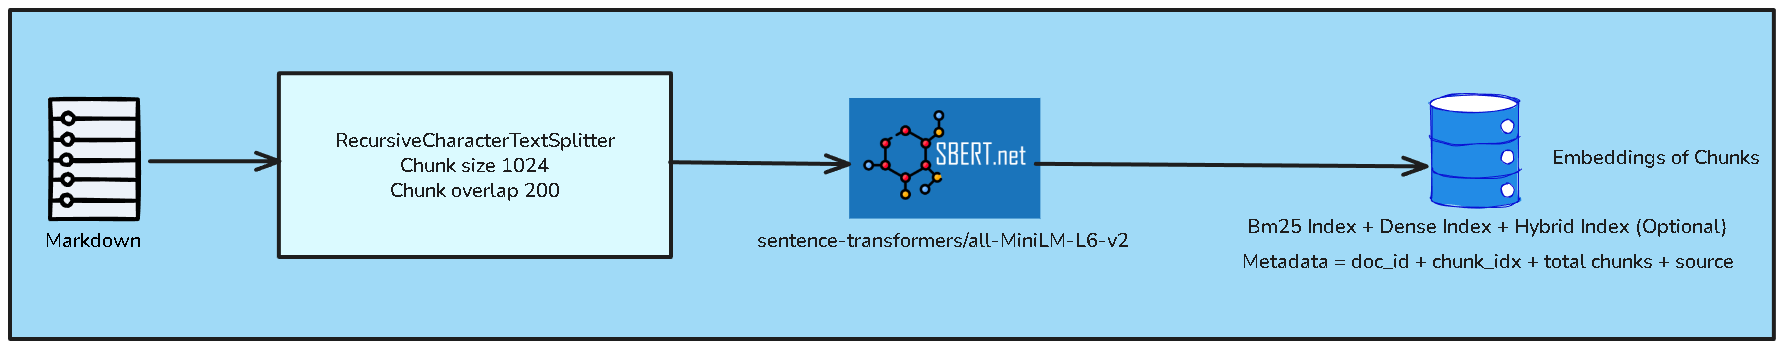
\includegraphics[width=1\textwidth]{img/pdz/20-textchunk.png}
    \caption[Textual Chunking and Embedding]{Textual Chunking and Embedding.}
    \label{fig:textchunk}
\end{figure}

Textual data is segmented into chunks to fit within the context window of the embedding models. 
The system employs the \texttt{RecursiveCharacterTextSplitter} with the configuration using a chunk size of 1024 characters with an overlap of 200 characters. 
This overlap ensures semantic continuity across chunk boundaries, preventing context loss for sentences that straddle the split point. 


\textbf{Text Vectorization (SBERT)}

Processed chunks are mapped to a high-dimensional vector space using the \textbf{Sentence-BERT (SBERT)} framework.
\begin{itemize}
    \item \textbf{Model}: \texttt{sentence-transformers/all-MiniLM-L6-v2}.
    \item \textbf{Output}: A 384-dimensional dense vector representing the semantic meaning of the text chunk.
    \item \textbf{Index Structure}: The embedding is stored alongside a composite metadata object containing:
    \begin{verbatim}
    {
      "doc_id": "unique_document_identifier",
      "chunk_idx": "integer_sequence_number",
      "total_chunks": "total_count_for_document",
      "source": "original_filename"
    }
    \end{verbatim}
\end{itemize}

\subsection{Visual Embedding Pipeline}

For documents rich in diagrams, charts, and complex layouts, the pipeline utilizes JPG images derived from the canonical PDF files.
% The system implements a ``1 Page = 1 Image'' conversion strategy. Each PDF page is rendered as a high-resolution JPEG image.
These intermediate image files are stored temporarily to facilitate the vision-based embedding process used by ColQwen, ensuring the model ``sees'' the document exactly as a human would.


The visual pathway processes the page images generated to enable multimodal retrieval.

\begin{figure}[H]
    \centering
    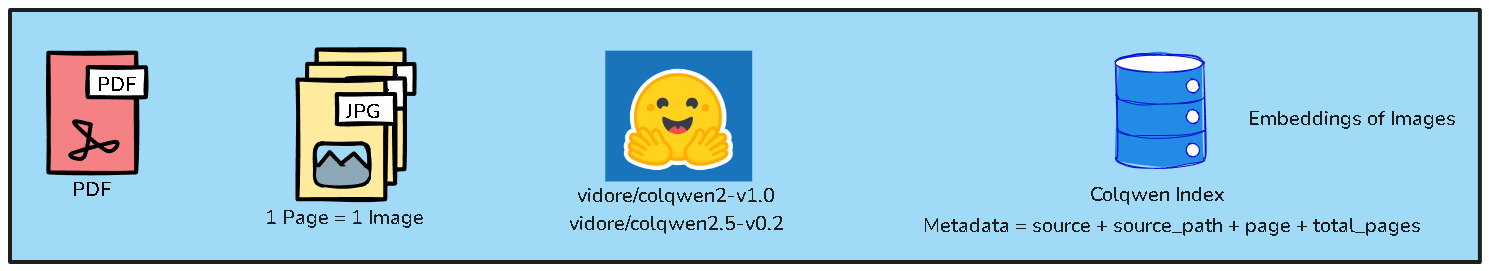
\includegraphics[width=1\textwidth]{img/pdz/21-visualemb.png}
    \caption[Visual Embedding (ColQwen)]{Visual Embedding (ColQwen).}
    \label{fig:visualemb}
\end{figure}

\textbf{Vision-Language Model}

The system integrates the \textbf{ColQwen} architecture (specifically \texttt{vidore/colqwen2-v1.0} or \texttt{v2.5}). Unlike standard OCR which strips layout, ColQwen encodes the visual semantics of the entire page.

\textbf{Visual Indexing}

\begin{itemize}
    \item \textbf{Embedding Process}: Each rasterized page image is passed through the ColQwen vision encoder to produce visual tokens.
    \item \textbf{Storage}: These embeddings are stored in a specialized ColQwen Index.
    \item \textbf{Metadata Schema}: Visual embeddings are tagged with precise location data:
    \begin{verbatim}
    {
      "source": "original_filename",
      "source_path": "file_system_path_to_pdf",
      "page": "page_number",
      "total_pages": "document_length"
    }
    \end{verbatim}
\end{itemize}

The text and visual embedding pipelines together constitute the dual-pathway indexing strategy, encoding documents into both dense semantic vectors and sparse token-level representations. The following section describes how these embeddings are organized, indexed, and queried within the Qdrant vector database and supporting storage layers.

\section{Indexing and Storage Architecture}

\subsection{Indexing Pipeline}

The consolidation and indexing pipeline transforms RAG-ready chunks into searchable indices through a dual-pathway approach:

\begin{table}[H]
\centering
\caption[Indexing Output Artifacts]{Artifacts produced by the indexing pipeline for each document.}
\label{tab:indexing_artifacts}
\resizebox{\textwidth}{!}{%
\begin{tabular}{@{}llll@{}}
\toprule
\textbf{Index Type} & \textbf{Data Structure} & \textbf{Storage Format} & \textbf{Query Mechanism} \\ \midrule
BM25 Index (Text) & Inverted index (term → docs) & Local BM25 file & Keyword matching, TF-IDF scoring \\
Dense Index (Text) & 384-dim embeddings (all-MiniLM-L6-v2) & Qdrant \texttt{edu\_text\_chunks} & Cosine similarity, HNSW search \\
Hybrid Index (Text) & RRF fusion results & Query-time computation & Combined BM25 + Dense scores \\
Visual Index (Images) & ColQwen multi-vectors (128 × $x$) & Qdrant \texttt{edu\_image\_pages} & Late-interaction MaxSim matching \\
Metadata Catalog & Document + chunk + image metadata & JSON files (S3) & Source tracking, citation generation \\
\bottomrule
\end{tabular}%
}
\end{table}

\textbf{Text Indexing Workflow}:
\begin{enumerate}
    \item Chunks from Stage 4 are encoded by SBERT (all-MiniLM-L6-v2) → 384-dimensional vectors
    \item BM25 inverted index built from chunk text (keyword search)
    \item Dense vectors indexed in Qdrant \texttt{edu\_text\_chunks} collection (semantic search)
    \item Hybrid index computed at query-time via RRF fusion for optimal recall
\end{enumerate}

\textbf{Visual Indexing Workflow}:
\begin{enumerate}
    \item PDF pages rasterized to JPEG (150 DPI, 1 page = 1 image)
    \item Each page encoded by ColQwen to multi-vector representation
    \item Vectors stored with minimal indexing (m=0 for HNSW bypass) to reduce memory overhead
    \item Query-time MaxSim computed on-demand for precision
\end{enumerate}

\textbf{Index Persistence Strategy}:

After indexing completes (Stage 4), the system:
\begin{enumerate}
    \item Pushes dense text embeddings to Qdrant \texttt{edu\_text\_chunks} collection with multi-tenant metadata
    \item Pushes visual embeddings to Qdrant \texttt{edu\_image\_pages} collection with page geometry references
    \item Stores BM25 index locally for fast keyword retrieval during search
    \item Qdrant provides persistent, scalable vector storage with built-in HNSW indices and MaxSim support
\end{enumerate}

\subsection{Search and Retrieval Pipeline}

The search pipeline orchestrates the concurrent retrieval of textual and visual information, optionally followed by generative synthesis. The workflow is designed for low-latency response times while maintaining high factual grounding.

\textbf{Retrieval Strategies}

The system supports three primary retrieval modalities to address different query types:
\begin{itemize}
    \item \textbf{Dense Retrieval}: Best for semantic understanding and handling synonymy. It uses the \texttt{all-MiniLM-L6-v2} model to match query embeddings against the Qdrant text collection.
    \item \textbf{Sparse Retrieval (BM25)}: Optimized for exact keyword matching, technical jargon, and specific entity retrieval.
    \item \textbf{Hybrid Retrieval}: Merges the results of dense and sparse retrievers using a weighted fusion approach. In Phase 2, the system utilizes an alpha weight of 0.5, providing a balanced trade-off between keyword precision and semantic recall.
\end{itemize}

\begin{figure}[H]
    \centering
    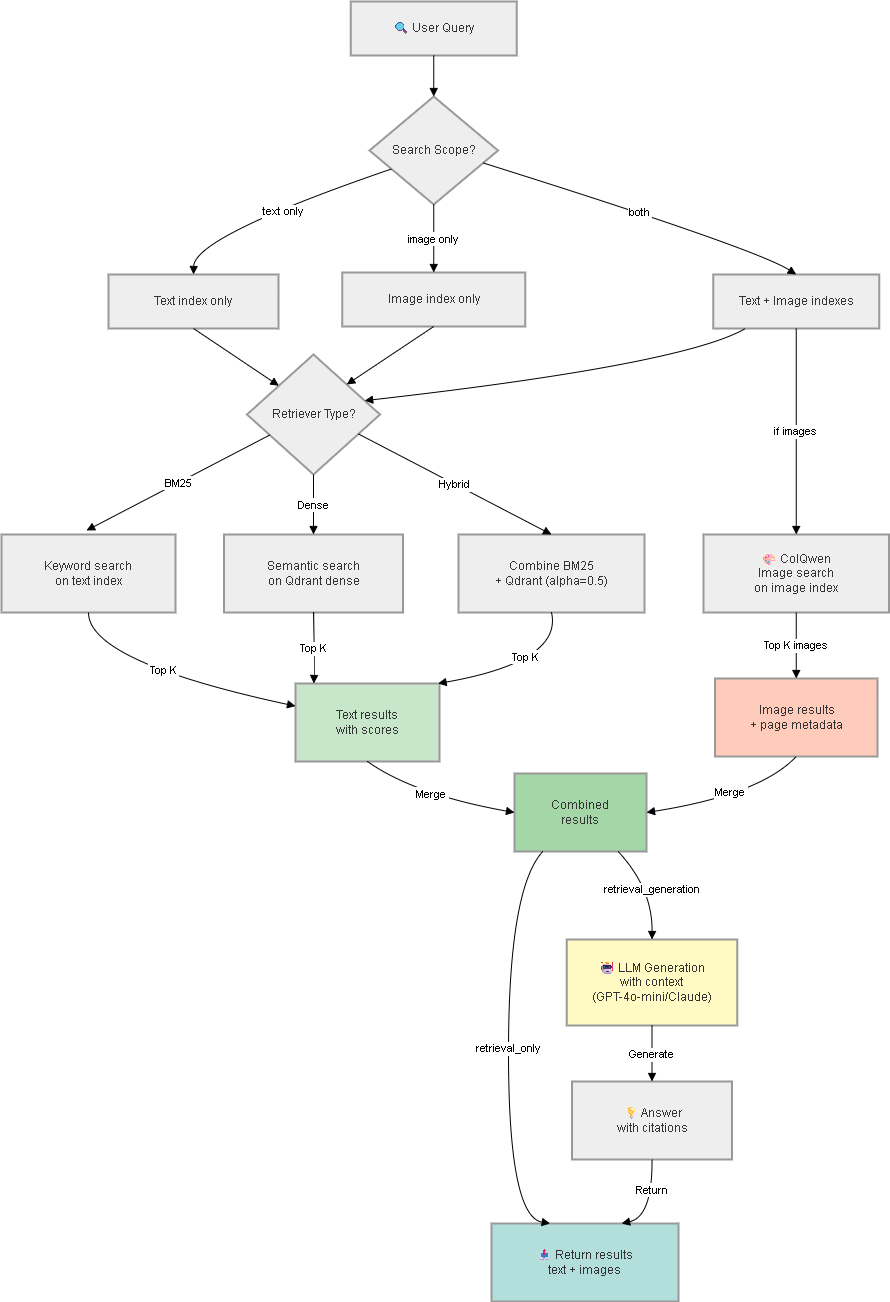
\includegraphics[width=0.9\textwidth]{img/pdz/Report 252 Diagram-Search Flow.drawio.png}
    \caption[Search and Retrieval Pipeline Flow]{Search and Retrieval Pipeline Flow.}
    \label{fig:search_flow}
\end{figure}

\textbf{Search Flow and Operational Modes}
As illustrated in Figure \ref{fig:search_flow}, the search orchestrator (\texttt{SearchService}) processes queries through a multi-step pipeline:
\begin{enumerate}
    \item \textbf{Decision Node: Search Scope}: Evaluates the query intent to target either the text index, image index, or a parallel multimodal retrieval.
    \item \textbf{Decision Node: Retriever Type}: Determines the retrieval algorithm (\texttt{BM25}, \texttt{Dense}, or \texttt{Hybrid}) based on the query complexity and user configuration.
    \item \textbf{Parallel Retrieval}:
    \begin{itemize}
        \item \textbf{Text Pathway}: Executes the selected retrieval logic on the text index, returning top $K$ chunks (default $K=10$).
        \item \textbf{Visual Pathway}: Executes a late-interaction search on the ColQwen image index if visual context is requested.
    \end{itemize}
    \item \textbf{Reranking (Optional)}: To further refine the results, a cross-encoder model (\texttt{bge-reranker-large}) can be applied to the merged candidate set (as illustrated in Figure \ref{fig:Reranker}). However, in the Phase 2 production environment, this step is \textbf{globally disabled by default} (\texttt{skip\_reranker=true}) to maintain sub-second retrieval latency.
    \item \textbf{Result Merging}: Contextualizes text chunks with their corresponding visual pages based on source metadata.
    \item \textbf{Mode Selection}:
    \begin{itemize}
        \item \textbf{Retrieval Only}: Immediately returns the merged text and image artifacts to the client.
        \item \textbf{Retrieval-Generation}: Injects the retrieved context into a Large Language Model to synthesize a grounded answer with citations.
    \end{itemize}
\end{enumerate}

\textbf{Response Structure and Metadata Tracking}

Every search response follows a standardized schema that integrates synthesized answers with granular metadata tracking. As defined in the system's design principles, every retrieved chunk preserves its provenance (source file, page, and chunk type) to ensure factual grounding. The response includes a detailed telemetry payload tracking retrieval latencies and model inference times, providing users with transparency regarding the ``source-of-truth'' for all generated answers.

\textbf{Generation Model and Fallback Routing}

The production answer generator is configured as a Bedrock-first model router. The preferred model for user-facing grounded QA is \textbf{Claude 4.7 Sonnet on AWS Bedrock}, selected because it provides strong long-context reasoning, reliable instruction following, and good citation behavior when answers must be grounded in retrieved text chunks and visual page evidence. Its main trade-off is higher cost and latency than smaller flash/nano models, so the system keeps lower-cost fallback routes for high-load or degraded-service conditions.

The fallback policy is:
\begin{itemize}
    \item \textbf{Primary}: \texttt{Claude 4.7 Sonnet} on AWS Bedrock for normal chat, summary, roadmap, and grounded QA generation.
    \item \textbf{First fallback}: \texttt{zai-glm-4.7-flash} through AWS Bedrock when lower latency/cost is preferred or the primary model is unavailable.
    \item \textbf{Second fallback}: \texttt{gpt-5.4-nano} for lightweight generation or external fallback paths.
\end{itemize}

For the evaluation pipeline, model roles are separated from production answer generation to reduce evaluator bias. Synthetic question and reference-answer generation uses \texttt{zai-glm-4.7-flash} through AWS Bedrock. Relevance and answer-quality judging uses \texttt{gpt-5.4-nano}. This separation prevents the same model family from both creating the benchmark item and judging the system output, while keeping evaluation cost manageable.


\subsection{Storage Architecture}

Phase 2 implements a \textbf{hybrid storage model} combining local processing cache with cloud canonical storage:

\begin{table}[H]
\centering
\caption[Hybrid Storage Architecture]{Local vs. Cloud storage division of responsibility.}
\label{tab:storage_architecture}
\resizebox{\textwidth}{!}{%
\begin{tabular}{@{}llll@{}}
\toprule
\textbf{Storage Tier} & \textbf{System} & \textbf{Content} & \textbf{Purpose} \\ \midrule
Local Cache & File system (fast SSD) & Processing artifacts (Stages 1-4) & Speed up pipeline processing \\
BM25 Index & Local file system & Inverted index for keyword search & Fast sparse retrieval \\
Vector Search & Qdrant Cloud & Dense text + visual embeddings & Scalable semantic retrieval \\
Cloud Documents & Amazon S3 & Raw documents, metadata, outputs & Durability, multi-tenancy \\
Session State & DynamoDB & Chat history, job queue state & Persistent conversation tracking \\
\bottomrule
\end{tabular}%
}
\end{table}

\textbf{Multi-Tenancy Isolation}:
\textbf{Hybrid Retrieval Integration}

The retrieval unifies these two streams. 
The Text and Visual indices can be queried simultaneously to return both relevant text snippets and their corresponding visual page contexts.

The index supports \textbf{Hybrid}, allowing for keyword precision and semantic recall, combining two distinct algorithms:

\begin{enumerate}
    \item \textbf{Sparse Retrieval (BM25)}: Utilizes keyword matching to capture exact terms and domain-specific jargon.
    \item \textbf{Dense Retrieval}: Utilizes vector embeddings (stored in Qdrant collections) to capture semantic meaning and context. The default embedding model is \texttt{all-MiniLM-L6-v2}.
\end{enumerate}

The system performs \textbf{Hybrid Fusion} using the Reciprocal Rank Fusion (RRF) or Distribution-Based Score Fusion algorithm, with a default \textbf{alpha weight of 0.5}, balancing keyword exactness with semantic similarity.

Scores from both retrievers are combined using Min-Max normalization and a weighted sum.




\section{Asynchronous Indexing Job System}

The Phase 2 system implements a \textbf{Redis-backed job queue} for managing asynchronous indexing operations, enabling non-blocking document processing while maintaining concurrent request limits and durable job state persistence.

\subsection{Purpose and Architecture}

Rather than forcing clients to wait for complete index updates, documents are queued for indexing via the \texttt{IndexingJobService}. This service coordinates three components:

\begin{itemize}
    \item \textbf{Redis Queue}: Transient job tracking with configurable TTL (default 3600 seconds). Each job receives a unique \texttt{job\_id} and tracks state transitions: \texttt{queued} $\rightarrow$ \texttt{processing} $\rightarrow$ \texttt{completed} or \texttt{failed}.

    \item \textbf{DynamoDB Persistence}: Optional backup to Amazon DynamoDB (\texttt{bk\_mind\_app\_jobs} table) for long-term durability and cross-service job history. Job snapshots include metadata, progress counters, and error details.

    \item \textbf{Concurrency Limits}: Per-user queue depth (\texttt{ASYNC\_INDEXING\_MAX\_PER\_USER}, default 3) and global queue depth (\texttt{ASYNC\_INDEXING\_MAX\_GLOBAL}, default 200) prevent resource exhaustion.
\end{itemize}

\subsection{Job Lifecycle and Progress Tracking}

Each indexing operation creates a job payload with status tracking. The service provides non-blocking status queries via \texttt{get\_job(job\_id)} and batch polling via \texttt{get\_jobs\_for\_user(user\_id)}, enabling frontend implementations to display real-time progress bars and resume interrupted indexing workflows.

\textbf{Fallback Behavior:} If Redis is unavailable and \texttt{ASYNC\_INDEXING\_FALLBACK\_TO\_BLOCKING=true}, the system gracefully degrades to synchronous processing, ensuring availability over responsiveness. Configuration is environment-driven (\texttt{ASYNC\_INDEXING\_ENABLED}, \texttt{REDIS\_URL}), supporting both container deployments and local development scenarios.

\textbf{Benefits of Asynchronous Indexing:}
\begin{itemize}
    \item \textbf{Non-blocking UX}: Clients receive immediate acknowledgment; indexing proceeds in background worker pools.
    \item \textbf{Durability}: DynamoDB persistence ensures jobs survive system restarts.
    \item \textbf{Multi-tenancy}: Per-user limits prevent single user's large jobs from starving others.
    \item \textbf{Observability}: Detailed progress metrics and error tracking support operational debugging.
\end{itemize}

With asynchronous job processing established as the infrastructure for long-running indexing operations, the system requires robust schema design and storage architecture to persist all processing artifacts, embeddings, and user state. The following section describes the three-tier hybrid storage architecture.


\section{Database Schema and Storage}
The system implementation requires a robust schema design to manage heterogeneous data including user interactions, processed documents, and high-dimensional vector representations. We utilize a \textbf{Hybrid Storage Architecture} to balance persistence, scalability, and low-latency retrieval across three specialized layers:

\begin{itemize}
    \item \textbf{Qdrant}: A specialized \textbf{Vector Database} and similarity search engine designed for storing and querying high-dimensional embeddings. Qdrant manages the multi-pathway vector representations of textual chunks and visual document pages, enabling semantic similarity matching and retrieval-augmented generation. It provides optimized search algorithms, filtering capabilities, and distributed indexing to maintain sub-second retrieval performance.
    \item \textbf{Amazon S3}: A highly scalable \textbf{Object Storage} service used to manage the complete lifecycle of document assets. It acts as the canonical source of truth, storing raw uploads, intermediate processing artifacts (e.g., extracted audio, keyframes), and final ``RAG-ready'' normalized documents. This layer ensures data durability and facilitates multi-tenant isolation through keyed prefixing.
    \item \textbf{Amazon DynamoDB}: A fully managed \textbf{NoSQL} database service that provides fast and predictable performance with seamless scalability. In our architecture, DynamoDB serves as the primary store for persistent metadata, user profile information, assessment results, conversational state, and system telemetry. Its schema-less nature allows for flexible data structures while its partitioned key-value access ensures low-latency operations.
\end{itemize}

\subsection{Schema Property Definitions}
Before detailing the specific collection structures, we define the properties utilized within our schema tables to ensure technical clarity.

\begin{table}[H]
    \centering
    \caption{Schema properties used in implementation documentation.}
    \label{tab:schema_props}
    \begin{tabular}{llp{8cm}}
        \toprule
        \textbf{Property} & \textbf{Description} & \textbf{Note} \\
        \midrule
        Field & Name of the attribute in the database & Mandatory. \\
        Type & The technical data format & String, Boolean, Enum, or Vector. \\
        Description & Purpose of the field within the system & Context for the specific attribute. \\
        Note & Structural role or indexing constraint & e.g., Primary Key, Partition Key, Sort Key. \\
        \midrule
        Dim & The length of the embedding vector & Mandatory for dense vector fields. \\
        Distance & The distance calculation for retrieval & Mandatory for vector indices (e.g., Cosine). \\
        \bottomrule
    \end{tabular}
\end{table}

\textbf{Key Concepts in DynamoDB Schema Design}

To effectively manage high-throughput data access and ensure efficient multi-tenant isolation, the system utilizes a robust primary key structure to uniquely identify each item in a table. Our architecture leverages both simple and composite primary keys:
\begin{itemize}
    \item \textbf{Primary Key}: The unique logical identifier for each item. In DynamoDB, the primary key is a role assigned to specific attributes and can take two forms:
    \begin{itemize}
        \item \textbf{Simple Primary Key (Partition Key only)}: Comprising just the partition key to uniquely identify items.
        \item \textbf{Composite Primary Key (Partition Key + Sort Key)}: Comprising both keys for more complex identification and sorting.
    \end{itemize}
    In the AWS Management Console, these are represented by their specific key descriptors rather than a single field named ``Primary Key.''
    \item \textbf{Partition Key (Hash Key)}: A mandatory attribute used by DynamoDB to distribute data across multiple physical partitions for horizontal scalability. In our schema, attributes like \texttt{user\_id} act as partition keys to ensure that all related data for a specific user is co-located.
    \item \textbf{Sort Key (Range Key)}: When combined with the partition key, the sort key creates a \textit{Composite Primary Key}. Items sharing the same partition key are stored in sorted order by their sort key value, enabling efficient range searches and ordered retrieval (e.g., chat messages by timestamp).
\end{itemize}

\subsection{Vector Storage (Qdrant)}
To support our Hybrid + Multimodal retrieval strategy, we segregate embeddings into dedicated Qdrant collections. Each collection is distinctly configured with dimensions and distance metrics tailored to the deployed embedding model architecture.

\textbf{Collection: \texttt{edu\_text\_chunks}}
Stores granular textual chunks extracted from structured Markdown documents. It utilizes a hybrid search approach, combining sparse keyword indexing with the following dense vector configuration.
\begin{table}[H]
    \centering
    \caption{Text Vector Collection Properties.}
    \label{tab:qdrant_text}
    \begin{tabular}{lp{1cm}p{1.8cm}p{5.5cm}}
        \toprule
        \textbf{Vector Name} & \textbf{Dim} & \textbf{Distance} & \textbf{Description} \\
        \midrule
        text & 384 & Cosine & Main text embeddings representing chunk semantics (e.g., via \texttt{all-MiniLM-L6-v2}). \\
        \bottomrule
    \end{tabular}
\end{table}

Each indexed text chunk retains critical metadata necessary for strict multi-tenant filtering and file attribution during generative retrieval:
\begin{table}[H]
    \centering
    \caption{Text Collection Schema Structure.}
    \label{tab:qdrant_text_schema}
    \begin{tabular}{llp{8cm}}
        \toprule
        \textbf{Field} & \textbf{Type} & \textbf{Note / Description} \\
        \midrule
        point\_id & UUID & Primary Key. Unique identifier mapped to the vector. \\
        \midrule
        chunk\_id & String & Unique string identifier for the block. \\
        user\_id & String & Tenancy boundary identifier. \\
        source & String & Original filename. \\
        text\_preview & String & Truncated preview of the chunk. \\
        storage\_uri & String & Cloud location of the chunk artifact. \\
        storage\_backend & String & Storage system (e.g., s3). \\
        \bottomrule
    \end{tabular}
\end{table}

\textbf{Collection: \texttt{edu\_image\_pages}}
Dedicated to storing high-order visual layouts. It leverages a unique multi-vector representation generated directly from the ColQwen vision-language model, enabling direct visual similarity searches against original PDF structures.
\begin{table}[H]
    \centering
    \caption{Image Vector Collection Properties.}
    \label{tab:qdrant_image}
    \begin{tabular}{lp{1.5cm}p{1.8cm}p{5.5cm}}
        \toprule
        \textbf{Vector Name} & \textbf{Dim} & \textbf{Distance} & \textbf{Description} \\
        \midrule
        colpali\_multivec & 128 $\times$ $x$ & Dot & Multi-vector representations (128 dims $\times$ $x$ visual tokens) for ColQwen late-interaction. \\
        \bottomrule
    \end{tabular}
\end{table}

\textbf{Visual Token Calculation Methodology}
The variable $x$ in the multi-vector representation represents the total number of distinct 128-dimensional embeddings stored per document page. Unlike standard text RAG that condenses an entire chunk into a single vector, the \texttt{ColQwen} architecture preserves granular spatial information by treating the page as an adaptive grid of patches. The value of $x$ is calculated as follows.

\begin{equation}
    x = \left( \lceil H / P \rceil \times \lceil W / P \rceil \right) + N_{special}
\end{equation}

where
\begin{itemize}
    \item \textbf{$x$}: The total count of vectors stored in the Qdrant collection for a single page.
    \item \textbf{$H$}: The height of the document page image after processing (typically 448 or 1024 pixels).
    \item \textbf{$W$}: The width of the document page image after processing (typically 448 or 1024 pixels).
    \item \textbf{$P$}: The patch size of the Vision Transformer (ViT) backbone, fixed at \textbf{14} for our implementation. Each $14 \times 14$ pixel area is vectorized into a single embedding.
    \item \textbf{$N_{special}$}: A technical constant (typically $< 10$) representing special delimiter tokens used by the multimodal LLM to frame the visual sequence.
\end{itemize}

For a standard processing resolution of $1024 \times 1024$ pixels, $x \approx 5,329$ vectors. This high-density representation ensures that fine-grained structural elements, such as table cells and chart labels, remain distinctly searchable during the late-interaction phase.

The visual index maintains geometric representations (height/width) alongside S3 references, allowing the orchestration layer to securely retrieve the original page images for multimodal language models:
\begin{table}[H]
    \centering
    \caption{Image Collection Schema Structure.}
    \label{tab:qdrant_image_schema}
    \begin{tabular}{llp{8cm}}
        \toprule
        \textbf{Field} & \textbf{Type} & \textbf{Note / Description} \\
        \midrule
        point\_id & UUID & Primary Key. Unique identifier mapped to the vector. \\
        \midrule
        user\_id & String & Tenancy boundary identifier. \\
        source & String & Original document name. \\
        source\_path & String & Absolute physical path of document. \\
        page & Integer & The structural page number. \\
        total\_pages & Integer & The total length of the PDF. \\
        image\_width & Integer & Pixel width of the page boundary. \\
        image\_height & Integer & Pixel height of the page boundary. \\
        storage\_uri & String & Cloud location of the rasterized image. \\
        storage\_backend & String & Storage system (e.g., s3). \\
        \bottomrule
    \end{tabular}
\end{table}

\subsection{Object Storage (Amazon S3)}
The system utilizes a dual-bucket object storage architecture to manage the lifecycle of document assets. This approach decouples raw ingestion from the downstream processing pipeline, ensuring data integrity and enabling scalable multi-tenancy.

\begin{figure}[H]
    \centering

    \begin{verbatim}
    S3/
    ├── ai-service-originals-dev/         # Bucket for raw document ingestion
    │   └── users/{uid}/                  # Logical user-tenant isolation
    │       ├── {doc_name}.pdf            # Original source document
    │       └── {doc_name}.pdf.metadata.json # Ingestion time & file provenance
    └── ai-service-processed-dev/         # Bucket for pipeline artifacts
        └── users/{uid}/
            ├── .processing_cache.json    # Idempotency and deduplication tracking
            ├── pipeline_stats.json       # Telemetry and processing performance
            ├── stage1_normalized/        # Standardized PDF & structured data
            │   ├── normalized_pdfs/      # Unified format for visual processing
            │   ├── excel_parsed/         # Structured tables from Office files
            │   ├── original_files/       # Internal reference copy
            │   └── normalization_metadata/
            ├── stage2_media_processed/   # Extracted audiovisual artifacts
            │   ├── extracted_audio/      # Raw audio for Whisper transcription
            │   ├── extracted_frames/     # Visual frames for late-interaction RAG
            │   ├── transcripts/          # ASR textual outputs
            │   └── media_metadata/       # Temporal feature mapping
            ├── stage3_document_processed/# Structural Markdown outputs
            │   ├── {doc_name}/
            │   │   ├── {doc_name}.md     # Cleaned semantic Markdown
            │   │   └── {doc_name}_metadata.json
            │   └── logs/                 # Granular stage-level logs
            │       ├── batch_summary_*.json
            │       └── processing_*.log
            ├── stage4_rag_ready/         # Optimized artifacts for RAG engine
            │   ├── {doc_name}/
            │   │   ├── {doc_name}.md     # Final semantic text
            │   │   ├── {doc_name}.pdf    # Optimized PDF for visual retrieval
            │   │   └── docling_additional/
            │   └── consolidation_stats.json
            └── retrieval/                # Secondary persistence for search indices
                ├── bm25_index.pkl        # Serialized sparse search index
                └── documents.json.pkl    # Document lookup table
    \end{verbatim}

    \caption{Amazon S3 Directory Structure Tree.}
    \label{fig:s3_tree}

\end{figure}

\begin{itemize}
    \item \textbf{Tenant Isolation}: Files are logically partitioned using the prefix for each user. This ensures strict data segregation and facilitates efficient cleanup of processing artifacts.
    \item \textbf{Dual-Bucket Lifecycle}: 
    \begin{itemize}
        \item \textbf{Originals Bucket}: Acts as the immutable source of truth for all raw user uploads.
        \item \textbf{Processed Bucket}: Stores all 7-stage normalized artifacts, metadata sidecars, and serialized indices. 
    \end{itemize}
    The orchestration layer manages the synchronization between these buckets, downloading assets to a local temporary workspace for high-speed processing before publishing the final RAG-ready documents to the Processed Bucket.
\end{itemize}

\textbf{Bucket 1: Originals Storage (\texttt{ai-service-originals-dev})}

This bucket acts as the primary ingestion point for all raw assets. To ensure strict user isolation, the bucket employs a keyed prefixing strategy:
\begin{enumerate}
    \item \textbf{User Partitioning}: \texttt{users/\{user\_id\}/} acts as the root prefix for all files owned by a specific tenant.
    \item \textbf{Asset Storage}: Each uploaded file (e.g., \texttt{lecture\_slides.pdf}) is stored alongside a corresponding \texttt{.metadata.json} sidecar. This sidecar contains provenance data, original filenames, and ingestion timestamps.
\end{enumerate}

\textbf{Bucket 2: Processed Storage (\texttt{ai-service-processed-dev})}

The processed bucket stores all intermediate and final artifacts generated by the 7-stage multimodal pipeline. This storage layer is optimized for high-speed retrieval by the Chat Assistant and Lecture Viewer services. The 7-stage design includes intelligent conditional routing where Stages 3b (Excel), 3c (DOCX), and 3d (PDF) run only if their respective custom-parsed outputs exist from Stage 1.

\begin{itemize}
    \item \textbf{Global Pipeline Tracking}: Located at the user root, the \texttt{.processing\_cache.json} and \texttt{pipeline\_stats.json} files manage idempotency and performance metrics, allowing the system to skip redundant processing steps.
    \item \textbf{Modular Artifact Hierarchy}: Processed data is organized into logical stages:
    \begin{itemize}
        \item \textbf{Stage 1 (Normalized)}: Contains standardized \texttt{normalized\_pdfs/}, extracted tables in \texttt{excel\_parsed/}, DOCX metadata in \texttt{docx\_parsed/}, PDF structure in \texttt{pdf\_parsed/}, and a copy of the \texttt{original\_files/} for traceability. It also includes \texttt{normalization\_stats.json} for tracking conversion success rates.
        \item \textbf{Stage 2 (Media Processed)}: Manages temporal and visual extraction artifacts with noise reduction (80Hz high-pass filter):
        \begin{itemize}
            \item \texttt{extracted\_audio/}: Noise-reduced audio tracks extracted from video containers for transcription.
            \item \texttt{extracted\_frames/}: Keyframes rendered from video streams for visual RAG indexing.
            \item \texttt{transcripts/}: Full textual outputs from the Whisper ASR engine applied to cleaned audio.
            \item \texttt{media\_metadata/}: JSON descriptors of temporal features and extraction parameters.
        \end{itemize}
        \item \textbf{Stage 3 (Document Processed)}: Stores structural parsing outputs from Docling for non-specialized file types, organized by document name:
        \begin{itemize}
            \item \texttt{\{doc\_name\}/}: Individual directories containing the structured \texttt{.md} file and its \texttt{\_metadata.json} sidecar.
            \item \texttt{logs/}: System-generated \texttt{.log} files and \texttt{batch\_summary.json} reports for auditability and error tracking.
        \end{itemize}
        \item \textbf{Stage 3b/3c/3d (Conditional Custom Parsers)}: If detected in Stage 1 outputs, these conditional stages output directly to stage4\_rag\_ready/:
        \begin{itemize}
            \item \textbf{Stage 3b (Excel)}: Custom XML parser with table-aware chunking (max 2000 chars), sheet metadata tracking.
            \item \textbf{Stage 3c (DOCX)}: Custom XML parser with heading-aware chunking, heading hierarchy tracking.
            \item \textbf{Stage 3d (PDF)}: Custom parser with heading-aware chunking, page-level references.
        \end{itemize}
        \item \textbf{Stage 4 (RAG Ready)}: The final consolidation layer merging outputs from all Stage 3 variants (Docling, Excel, DOCX, PDF) into unified RAG-ready assets partitioned by document topic. Each document directory includes:
        \begin{itemize}
            \item \texttt{chunks.json}: Consolidated text chunks with metadata tracking source type (docx|pdf|excel|media)
            \item \texttt{metadata.json}: Provenance and structural metadata from all processing stages
            \item \texttt{images/}: Unified visual assets from all stages (extracted images, page previews, etc.)
            \item \texttt{transcripts/}: Links to media transcripts from Stage 2 (if applicable)
        \end{itemize}
        It includes \texttt{consolidation\_stats.json} to track the integrity of the final output set.
        \item \textbf{Retrieval Index}: Dedicated storage for serializable indices, including the \texttt{bm25\_index.pkl} and \texttt{documents.json.pkl} map used for efficient lookup.
    \end{itemize}
\end{itemize}

\subsection{Metadata and State Schemas}
Stateful operations are managed through a unified cloud architecture, primarily utilizing \textbf{Amazon DynamoDB} for high-throughput chat logging, user identity profiles, and assessment outcomes. 

\begin{itemize}
    \item \textbf{User Profile Table}: Stores core identity profiles, education levels, and selected personas.
    \item \textbf{Chatbot Sessions Table}: Organizes chat histories per user for stateful UI rendering.
    \item \textbf{Chatbot Messages Table}: Persists individual conversational turns and multimodal traces.
    \item \textbf{Quiz Results Table}: Facilitates academic tracking by storing generated assessment outcomes.
    \item \textbf{Feedback Table}: Captures user sentiment and tracks AI-driven quality analysis.
    \item \textbf{App Usage Table}: Logs granular telemetry for every AI-driven request and tracks costs.
    \item \textbf{App Jobs Table}: Acts as an asynchronous task registry for long-running extractions.
\end{itemize}

For detailed schema definitions and field information, please refer to Appendix \ref{chap:database_schemas}.

\section{Core API Services}
The backend architecture exposes a comprehensive suite of RESTful API endpoints and Server-Sent Events (SSE) streams to orchestrate the multimodal processing pipeline and conversational interfaces. The summary of core endpoints and their primary use cases are listed below:

\begin{itemize}
    \item \textbf{Upload Files} [\texttt{POST /api/upload}]: Ingests raw document assets into the storage backend, enabling high-concurrency multi-file uploads.
    \item \textbf{Run Pipeline} [\texttt{POST /api/process}]: Orchestrates the 7-stage multimodal extraction and normalization pipeline for document parsing.
    \item \textbf{Build Index} [\texttt{POST /api/index}]: Synchronizes extracted artifacts into Qdrant vector collections and BM25 sparse indices for search.
    \item \textbf{Knowledge Explorer} [\texttt{POST /api/search}]: Facilitates hybrid (dense + sparse) retrieval and visual context rendering for queries.
    \item \textbf{Summary Generation} [\texttt{POST /api/insights/summary}]: Synthesizes structured document outputs into context-aware abstracts and targeted summaries.
    \item \textbf{Lecture Viewer} [\texttt{GET /api/processed-file}]: Serves processed artifacts (e.g., Markdown, images) for inline previewing securely.
    \item \textbf{Learning Path} [\texttt{POST /api/insights/learning-roadmap}]: Generates educational progressions and prerequisite roadmaps based on user goals.
    \item \textbf{Multiple Choice Questions} [\texttt{POST /api/insights/mcq}]: Automates knowledge validation by generating tailored quizzes with rationales.
    \item \textbf{Chat Assistant} [\texttt{POST /api/chat/stream}]: Manages stateful conversational RAG interactions, streaming AI responses with session history.
    \item \textbf{Feedbacks} [\texttt{POST /api/feedback}]: Captures granular user sentiment on AI behavior and drives asynchronous quality analysis.
\end{itemize}

For detailed API specifications including request headers, payloads, and response structures, please refer to Appendix \ref{chap:api_specs}.

\section{System Deployment}

The system is deployed as a cloud-native application on a hybrid multi-cloud infrastructure, leveraging the scalability and reliability of AWS services alongside specialized vector and database backends. This deployment model ensures high availability, low-latency response times, multi-tenant isolation, and high-performance processing of multimodal assets. The architecture follows a microservices paradigm, with distinct separation between API serving, compute-intensive inference, persistent storage, and managed vector search. This decoupling allows each component to scale independently based on demand, optimizing both performance and cost.

The deployment strategy prioritizes both operational excellence and security. Every code change undergoes automated testing and validation before reaching production. Containerization ensures environment parity between development and production environments, eliminating the ``works on my machine'' problem that plagues many deployments. Encryption is enforced at multiple layers: in-transit via TLS, at-rest via AWS-managed encryption keys, and for application data via JWT-based authentication. The infrastructure also integrates comprehensive observability through AWS CloudWatch, enabling real-time monitoring of system health and rapid incident response.

\begin{figure}[H]
    \centering
    \includegraphics[width=1\textwidth]{img/pdz/28-Deployment Diagram_v4.png}
    \caption[System Deployment Architecture]{System Deployment Architecture Diagram.}
    \label{fig:deployment_diagram}
\end{figure}

As illustrated in Figure~\ref{fig:deployment_diagram}, the deployment architecture comprises five integrated components:

\textbf{CI/CD Component:} The pipeline is fully automated via GitHub Actions. On every push to \texttt{main} or \texttt{develop}, the workflow builds Docker images for the frontend and backend, tags them with the commit SHA for traceability, and pushes them to Amazon ECR (Elastic Container Registry). AWS Secrets Manager stores all credentials and environment variables, injected securely at runtime.

\textbf{AWS VPC - Public and Private Subnets:} All user traffic first passes through \textbf{AWS WAF} (Web Application Firewall) for threat filtering, then through \textbf{AWS CloudFront} CDN (which injects X-Origin-Key headers for origin verification) before reaching the Application Load Balancer in the public subnet. A NAT Gateway handles outbound traffic for private-subnet services. The \textbf{Private Subnets App Tier} contains an \textbf{AWS ECS Cluster} running two services: the Frontend Service (React, containerized) and the Backend Service (FastAPI RAG pipeline), each with their own ECS Task Definition, IAM Task Role, Auto Scaling policies, and CloudWatch alarms for health monitoring. The backend also integrates with \textbf{Amazon Bedrock} for LLM API streaming.

\textbf{Data Component:} Persistent state is managed across three AWS managed services: \textbf{Amazon S3} (document and artifact storage with SSE-S3 encryption, block public access), \textbf{Amazon SQS} (job queue for asynchronous indexing tasks), and \textbf{Amazon DynamoDB} (chat session and message persistence with SSE encryption). All services enforce block public access policies.

\textbf{Inference Tier:} Compute-intensive AI inference is offloaded to a dedicated \textbf{EC2 Auto Scaling Group} in a private subnet. Each EC2 instance runs Docker Compose to orchestrate the GPU Model Server, hosting \textbf{Whisper Large-v3} for audio transcription and \textbf{Qwen2-VL} (ColQwen 2.5) for visual embedding. The tier also integrates with \textbf{Amazon SageMaker} for scalable model inference, ensuring the main ECS application tier remains responsive during heavy batch processing.

\textbf{External Services:} \textbf{Qdrant Cloud} provides the managed vector database for both text and visual embedding collections. An \textbf{Observability Component} aggregates logs and metrics via AWS CloudWatch, CloudTrail audit logs, X-Ray distributed tracing, and an S3 bucket for log archival.

\subsection{CI/CD Pipeline (GitHub Actions)}

The system implements a fully automated \textbf{Continuous Integration and Continuous Deployment (CI/CD)} pipeline using \textbf{GitHub Actions}. This ensures that every code change is validated, containerized, and deployed with minimal manual intervention, reducing human error and accelerating the development cycle.

\textbf{Pipeline Architecture and Workflow}

The CI/CD pipeline is event-driven, triggered automatically upon a code push to the \texttt{main} (production) or \texttt{develop} (staging) branches. This event-driven model enforces a strict separation between development experimentation (on feature branches) and validated, deployable code (on \texttt{develop} and \texttt{main}). The pipeline enforces consistency and repeatability: the same exact build process that generated a tested artifact on a developer's local machine is executed in the GitHub Actions runner, ensuring no environmental drift.

The pipeline consists of multiple sequential stages that validate code quality before deployment:

\begin{enumerate}
    \item \textbf{Code Checkout and Preparation}: The workflow checks out the repository code and establishes secure AWS credentials using OpenID Connect (OIDC). This eliminates the need to store long-lived AWS access keys in GitHub Secrets, significantly reducing credential exposure risk.
    
    \item \textbf{Build Stage}: The application code is compiled and containerized. For the frontend (React), this involves transpilation of TypeScript/JSX to optimized JavaScript bundles. For the backend (FastAPI), dependencies are resolved and the application is packaged along with all required Python packages.
    
    \item \textbf{Container Registry Ingestion}: The built container images are pushed to \textbf{Amazon Elastic Container Registry (ECR)}, AWS's managed container registry. Each image is tagged with multiple identifiers: the Git commit SHA for precise version tracking, a branch name (e.g., \texttt{develop}, \texttt{main}), and the timestamp of the build. This multi-tag strategy enables rapid identification of which code version is running in production and facilitates quick rollbacks if necessary.
    
    \item \textbf{Orchestration Update}: For deployments to \texttt{main} (production), the workflow creates a new task definition in Amazon ECS with the new image reference. It then updates the corresponding service to use this task definition, triggering a rolling update. The rolling update strategy ensures zero-downtime deployments: new containers start with the new image while old containers are gradually drained of traffic and terminated only after health checks pass.
    
    \item \textbf{Verification}: CloudWatch alarms monitor the health of the newly deployed containers. If any container fails its health check within a configurable window, the deployment is automatically rolled back to the previous known-good version.
\end{enumerate}

\textbf{Security and Secrets Management}

All sensitive data-database credentials, API keys, LLM authentication tokens-is stored in \textbf{AWS Secrets Manager} rather than in the GitHub repository or environment variables. During the CI/CD pipeline execution, these secrets are injected as environment variables into the container at runtime, never exposed in logs or stored on disk. This secret rotation mechanism ensures that compromised credentials can be invalidated without redeploying the entire application.

The use of OIDC for AWS credential exchange (rather than long-lived IAM access keys) further hardens the pipeline. OIDC tokens are short-lived, automatically generated by GitHub for each workflow run, and scoped to specific AWS permissions (least privilege). This eliminates the risk of leaked credentials persisting indefinitely in GitHub's secret storage.

\subsection{Containerization and Orchestration}

To ensure environment parity across development, staging, and production environments, the system utilizes a modern containerization stack built on Docker and AWS managed services. This approach encapsulates application logic, dependencies, and configurations into portable, immutable units that can be deployed consistently across any infrastructure.

\textbf{1. Containerization (Docker)}

The backend and frontend applications are packaged as lightweight \textbf{Docker} containers. Each container is a self-contained execution environment that includes the application code, all runtime dependencies (e.g., Python packages via pip, Node.js modules via npm), system libraries, and configuration files. By bundling everything into a single image, Docker eliminates the problem of ``it works on my machine but not on the server'': if the container runs locally on a developer's laptop, it will run identically on a production server, because the entire environment is frozen in the image.

\textbf{Benefits of Containerization}:
\begin{itemize}
    \item \textbf{Reproducibility}: The same image runs the same way everywhere, eliminating environmental drift and configuration drift that plague non-containerized deployments.
    \item \textbf{Isolation}: Each container is isolated from others, preventing interference (e.g., one container's dependency conflict cannot break another).
    \item \textbf{Rapid Scaling}: New containers can be spawned in seconds, enabling the system to handle traffic spikes without lengthy provisioning delays.
    \item \textbf{Simplified Debugging}: Developers can pull the exact same image used in production to reproduce issues locally.
\end{itemize}

\textbf{2. Registry (Amazon Elastic Container Registry)}

All built container images are versioned and stored in \textbf{Amazon Elastic Container Registry (ECR)}, AWS's fully managed container image registry. Rather than storing images on developer machines or public registries (which pose security risks), ECR provides a private, encrypted repository for all application images.

The system utilizes a sophisticated multi-tag strategy for each image:
\begin{itemize}
    \item \textbf{Commit SHA}: The Git commit hash (e.g., \texttt{a3f7d2c}) uniquely identifies the exact source code version that produced the image, enabling precise traceability and rollback.
    \item \textbf{Branch Tag}: Tags like \texttt{develop}, \texttt{main}, \texttt{staging} allow quick reference to the latest image for a given branch without needing to know the commit hash.
    \item \textbf{Build Timestamp}: Each image is also tagged with the build timestamp (e.g., \texttt{2026-05-05-14:32:18}), facilitating chronological tracking of deployments.
\end{itemize}

This multi-tag approach provides auditability and rapid rollback capabilities. If a newly deployed version causes issues, operations teams can immediately identify the previous known-good version and redeploy it by referencing its commit SHA or timestamp tag.

\textbf{3. Orchestration (Amazon Elastic Container Service)}

The runtime environment is managed by \textbf{Amazon Elastic Container Service (ECS)}, a fully managed container orchestration platform. ECS abstracts away the complexity of managing a cluster of servers and instead presents a simple, declarative interface: ``I want 2 instances of the backend service to always be running.''

\textbf{Cluster Management}: The application is deployed into a managed ECS cluster (\texttt{rag-pipeline-cluster}) that handles the complexity of service discovery and health monitoring. Each service in the cluster is automatically assigned a DNS name (e.g., \texttt{backend-service.rag-pipeline-cluster}), allowing frontend and backend services to communicate without hardcoding IP addresses. If a container becomes unhealthy (e.g., crashes or stops responding), ECS automatically detects this via health checks and launches a replacement container to maintain the desired service count.

\textbf{Task Definitions}: ECS uses declarative \textbf{task definitions} to specify the runtime requirements of each service:
\begin{itemize}
    \item \textbf{CPU and Memory}: Each task is allocated specific CPU units and RAM (e.g., the backend service might request 0.5 vCPU and 512 MB RAM). ECS uses this to make intelligent scheduling decisions, packing tasks onto EC2 instances without exceeding capacity.
    \item \textbf{Environment Variables}: Configuration specific to the deployment environment (e.g., \texttt{API\_KEY}, \texttt{DATABASE\_URL}, \texttt{LLM\_MODEL\_NAME}) is injected at runtime from AWS Secrets Manager, eliminating the need to hardcode secrets in images.
    \item \textbf{Logging Configuration}: Each task is configured to stream logs to AWS CloudWatch, creating a centralized audit trail and enabling rapid debugging of production issues.
    \item \textbf{IAM Task Role}: Each ECS task is assigned a fine-grained IAM role that grants permissions only to the AWS services it actually needs (e.g., the backend task role grants \texttt{s3:GetObject}, \texttt{s3:PutObject} for S3 access, but denies access to other AWS resources). This principle of least privilege prevents one compromised service from accessing resources it shouldn't.
\end{itemize}

\textbf{High Availability and Auto-Scaling}: ECS ensures that the desired number of containers are always running through automated health monitoring. If a container fails its health check (e.g., the FastAPI application becomes unresponsive), ECS automatically terminates the unhealthy container and launches a replacement. For traffic spikes, the system is configured with auto-scaling policies: if CPU utilization or request count exceeds a threshold (e.g., 70\% CPU), ECS automatically increases the number of running tasks to distribute the load. Conversely, during quiet periods, idle tasks are scaled down to optimize costs.

The combination of containerization, a private registry, and orchestration creates a deployment pipeline that is simultaneously secure (secrets never exposed), scalable (scale up in seconds), reliable (automatic recovery from failures), and auditable (every deployment is tracked by commit hash and timestamp).

\section{Security Architecture and Implementation}

The overall security architecture design and threat model are presented in Chapter~5 (Proposed Solution), Section~\ref{sec:security_arch}. This section details the implementation, configuration parameters, and operational monitoring of each security tier.

BK-MInD implements a comprehensive, multi-layered security architecture designed to protect sensitive educational data, ensure platform availability, and maintain a safe learning environment for all users. This security framework operates across three distinct tiers: infrastructure-level protection via AWS Web Application Firewall (WAF), application-level content safety through AWS Bedrock Guardrails, and data-level encryption through industry-standard protocols. The implementation has been validated against industry standards including OWASP Top 10 threats and undergoes continuous monitoring to ensure protection against emerging threats.

\subsection{Infrastructure-Level Security: AWS Web Application Firewall}

\textbf{WAF Architecture and Deployment}

The BK-MInD application is protected by AWS WAF, a managed Web Application Firewall service that operates at layer 7 (application layer) of the OSI model. Unlike traditional firewalls that operate at network layers 3-4, AWS WAF understands HTTP/HTTPS protocols and analyzes the semantic meaning of requests, enabling sophisticated protection against application-level attacks. The WAF is deployed as a Protection Pack with identifier \texttt{37762d47-d786-40c2-ab94-878be6e4e0ee} in the US West 2 region, associated with the Application Load Balancer (ALB) that sits in front of all containerized backend services.

By placing the WAF at the ALB level, all inbound traffic is filtered before reaching application servers, providing early detection and blocking of malicious requests. The WAF operates using a default ``Allow'' action, meaning requests are allowed unless they match explicit protection rules. This approach balances security with legitimate user experience.

\begin{figure}[H]
    \centering
    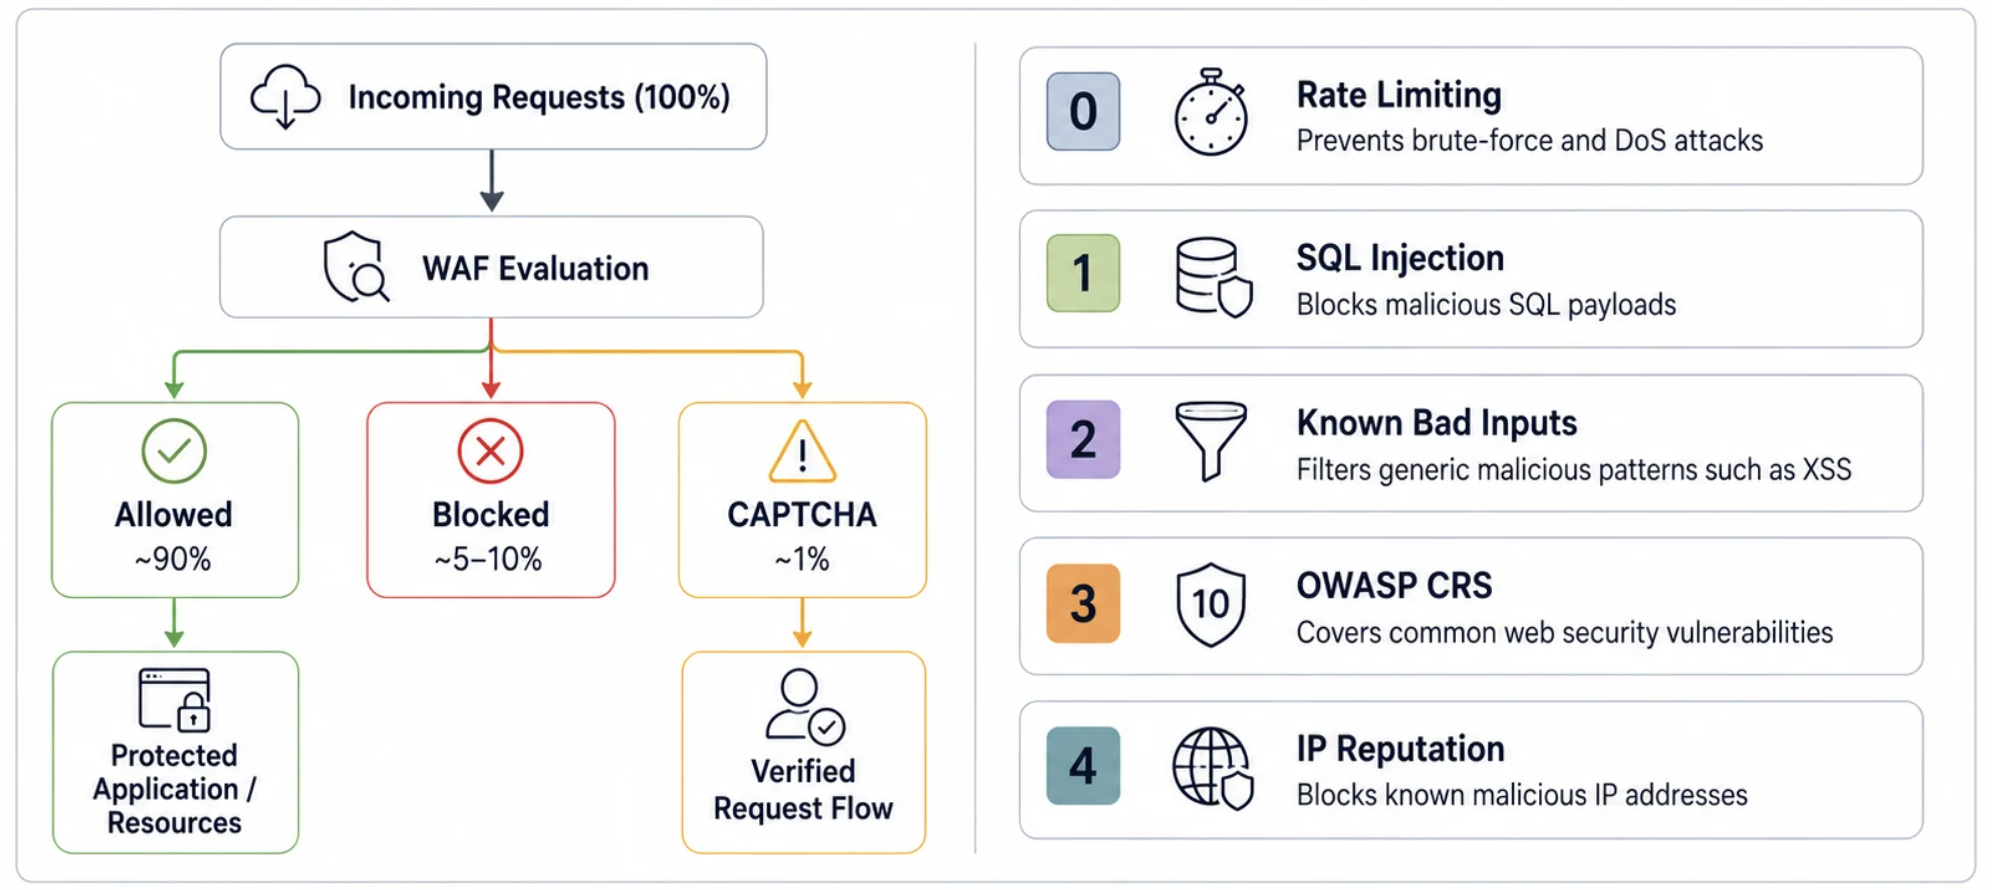
\includegraphics[width=1\textwidth]{img/pdz/47-aws-waf.png}
    \caption[AWS Web Application Firewall Architecture]{AWS Web Application Firewall (WAF) deployment architecture protecting the BK-MInD ALB.}
    \label{fig:waf_architecture}
\end{figure}

\textbf{Protection Rules and Threat Model}

The protection pack implements five distinct security rules, each targeting a specific attack category:

\begin{enumerate}
    \item \textbf{Rate Limiting (Priority 0):} Blocks any IP exceeding 2,000 requests within a 5-minute window. This protects against brute-force attacks on the login endpoint, credential stuffing attacks, and volumetric DDoS attacks from single or small numbers of compromised machines. Legitimate users typically generate 10-20 requests per minute during active sessions, well below this threshold.

    \item \textbf{SQL Injection Detection (Priority 1):} Analyzes all request parameters (query strings, POST body, cookies, headers) for SQL attack patterns. While BK-MInD uses DynamoDB rather than SQL databases, this rule protects against injection attacks that may exploit parsing vulnerabilities or authentication mechanisms. Detection uses machine learning and signature-based approaches with $<1\%$ false positive rate.

    \item \textbf{Known Bad Inputs (Priority 2):} Detects exploitation attempts from known attack tools and toolkits, including Log4Shell vulnerability exploits, Struts2 RCE attempts, PHP probes, and directory traversal attacks. AWS updates signatures weekly as new CVEs are disclosed.

    \item \textbf{Common Rule Set (Priority 3):} Implements the AWS adaptation of OWASP ModSecurity Core Rule Set (CRS) v3.2, providing industry-standard web application protection. Covers Cross-Site Scripting (XSS), Local File Inclusion (LFI), Remote Code Execution (RCE), and malformed HTTP requests.

    \item \textbf{IP Reputation List (Priority 4):} Leverages the Amazon IP Reputation List-a continuously updated database of IPs known for malicious activity including botnet C\&C servers, malware distribution endpoints, and credential stuffing sources. Updated daily with false positive rate $<0.1\%$.
\end{enumerate}

\textbf{Capacity and Performance}

The WAF uses a consumption model based on Web ACL Capacity Units (WCUs). The current configuration consumes 1,129 WCUs out of a maximum capacity of 5,000 WCUs, representing 22.6\% utilization. This leaves significant headroom (3,871 WCUs) for future security enhancements. Performance testing shows that WAF processing adds only 1-5 milliseconds per request-less than 0.1\% of typical backend processing time (100-500ms) and imperceptible to end users.

\begin{table}[H]
    \centering
    \caption{WAF Capacity Utilization and Cost.}
    \label{tab:waf_capacity}
    \scalebox{0.85}{
    \begin{tabular}{lrr}
        \toprule
        \textbf{Metric} & \textbf{Current} & \textbf{Capacity/Cost} \\
        \midrule
        WCU Utilization & 1,129 & 5,000 (22.6\%) \\
        Rate Limit Rule & 200 WCU & $\sim$\$0.30/month \\
        SQL Injection Rule & 200 WCU & $\sim$\$0.30/month \\
        Known Bad Inputs & 200 WCU & $\sim$\$0.30/month \\
        Common Rule Set & 400 WCU & $\sim$\$0.60/month \\
        IP Reputation & 129 WCU & $\sim$\$0.19/month \\
        \midrule
        Total WAF Cost & & $\sim$\$15/month (10M req/mo) \\
        \bottomrule
    \end{tabular}
    }
\end{table}

\textbf{Request Processing Flow}

When a request arrives at the ALB, the WAF sequentially evaluates it against all rules in priority order. If the request exceeds rate limits, exhibits SQL injection patterns, matches known bad inputs, contains attack signatures from the common rule set, or originates from a reputation-listed IP, it is immediately blocked with HTTP 403 response. Otherwise, the default ``Allow'' action applies and the request is forwarded to application services. All blocked requests are logged with full details for security monitoring.

The WAF also implements a challenge mechanism using CAPTCHA for suspicious but not definitively malicious requests. Upon successful CAPTCHA completion, users receive a token valid for 300 seconds, allowing legitimate users to proceed while filtering automated attacks.

\begin{figure}[H]
    \centering
    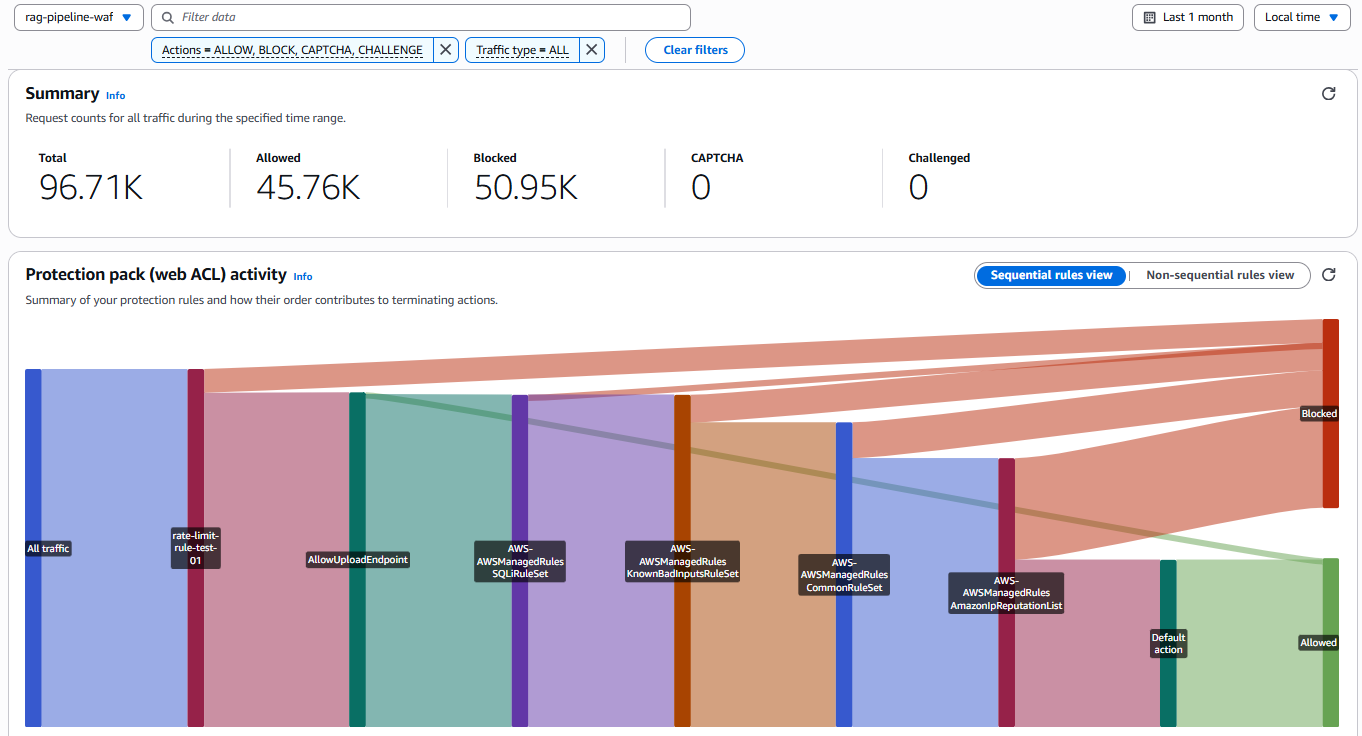
\includegraphics[width=1\textwidth]{img/pdz/50-waf-summary-view.png}
    \caption[WAF Summary Dashboard]{AWS WAF summary dashboard showing request volume, blocked requests, and CAPTCHA challenges.}
    \label{fig:waf_dashboard}
\end{figure}

\textbf{Monitoring and Observability}

The WAF exports detailed metrics to AWS CloudWatch including counts of allowed requests, blocked requests, and CAPTCHA challenges issued. BK-MInD is configured to alert operations teams when security thresholds are exceeded:
\begin{itemize}
    \item Alert if $>10\%$ of requests are blocked (indicating possible attack or misconfiguration)
    \item Rate-limit alert if $>100$ requests blocked per minute (indicating possible DDoS)
    \item CAPTCHA alert if $>1\%$ of requests require verification (indicating bot activity)
\end{itemize}

Blocked requests are logged to CloudWatch Logs for forensic analysis, including request details, matched rule, source IP, and timestamp. This enables security engineers to understand attack patterns and adjust configurations accordingly.

\begin{figure}[H]
    \centering
    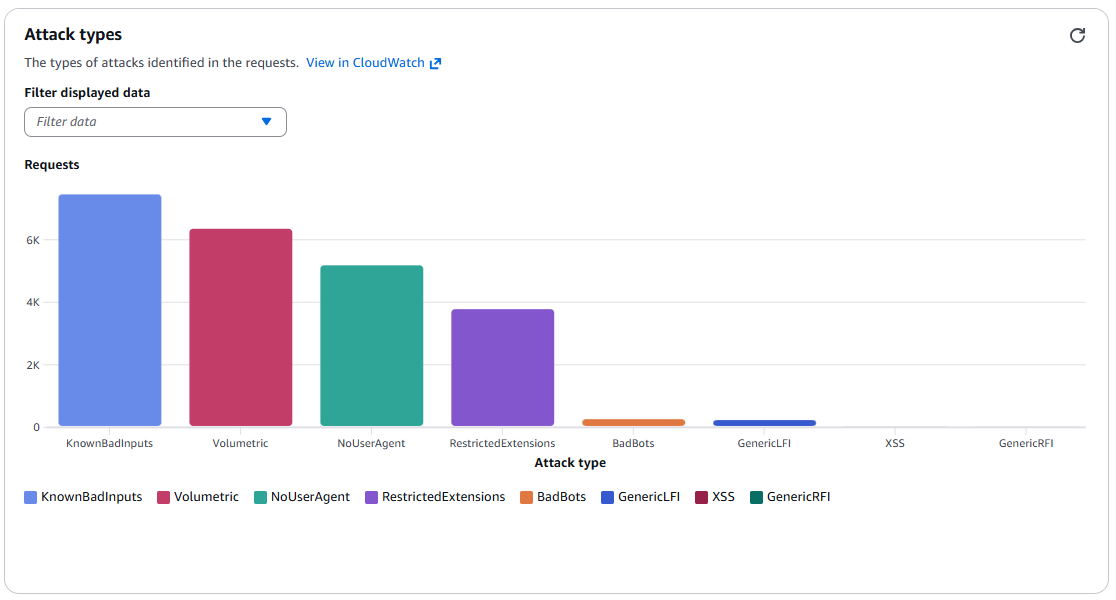
\includegraphics[width=1\textwidth]{img/pdz/51-waf-attack-type.png}
    \caption[WAF Attack Type Distribution]{WAF dashboard showing distribution of detected attack types.}
    \label{fig:waf_attacks}
\end{figure}

% \newpage

\subsection{Application-Level Security: AWS Bedrock Guardrails}

\textbf{Content Safety and Filtering}

While AWS WAF protects against technical network-layer attacks, BK-MInD requires additional protection at the application layer to ensure generated content remains appropriate for educational environments. This is implemented through AWS Bedrock Guardrails, which filter both user input (prompts) and model-generated output (responses) before reaching users. The guardrail configuration (\texttt{42ay3u3pr8vr}) is integrated into all Bedrock model inference calls, ensuring every interaction with AI models is protected.

\begin{figure}[H]
    \centering
    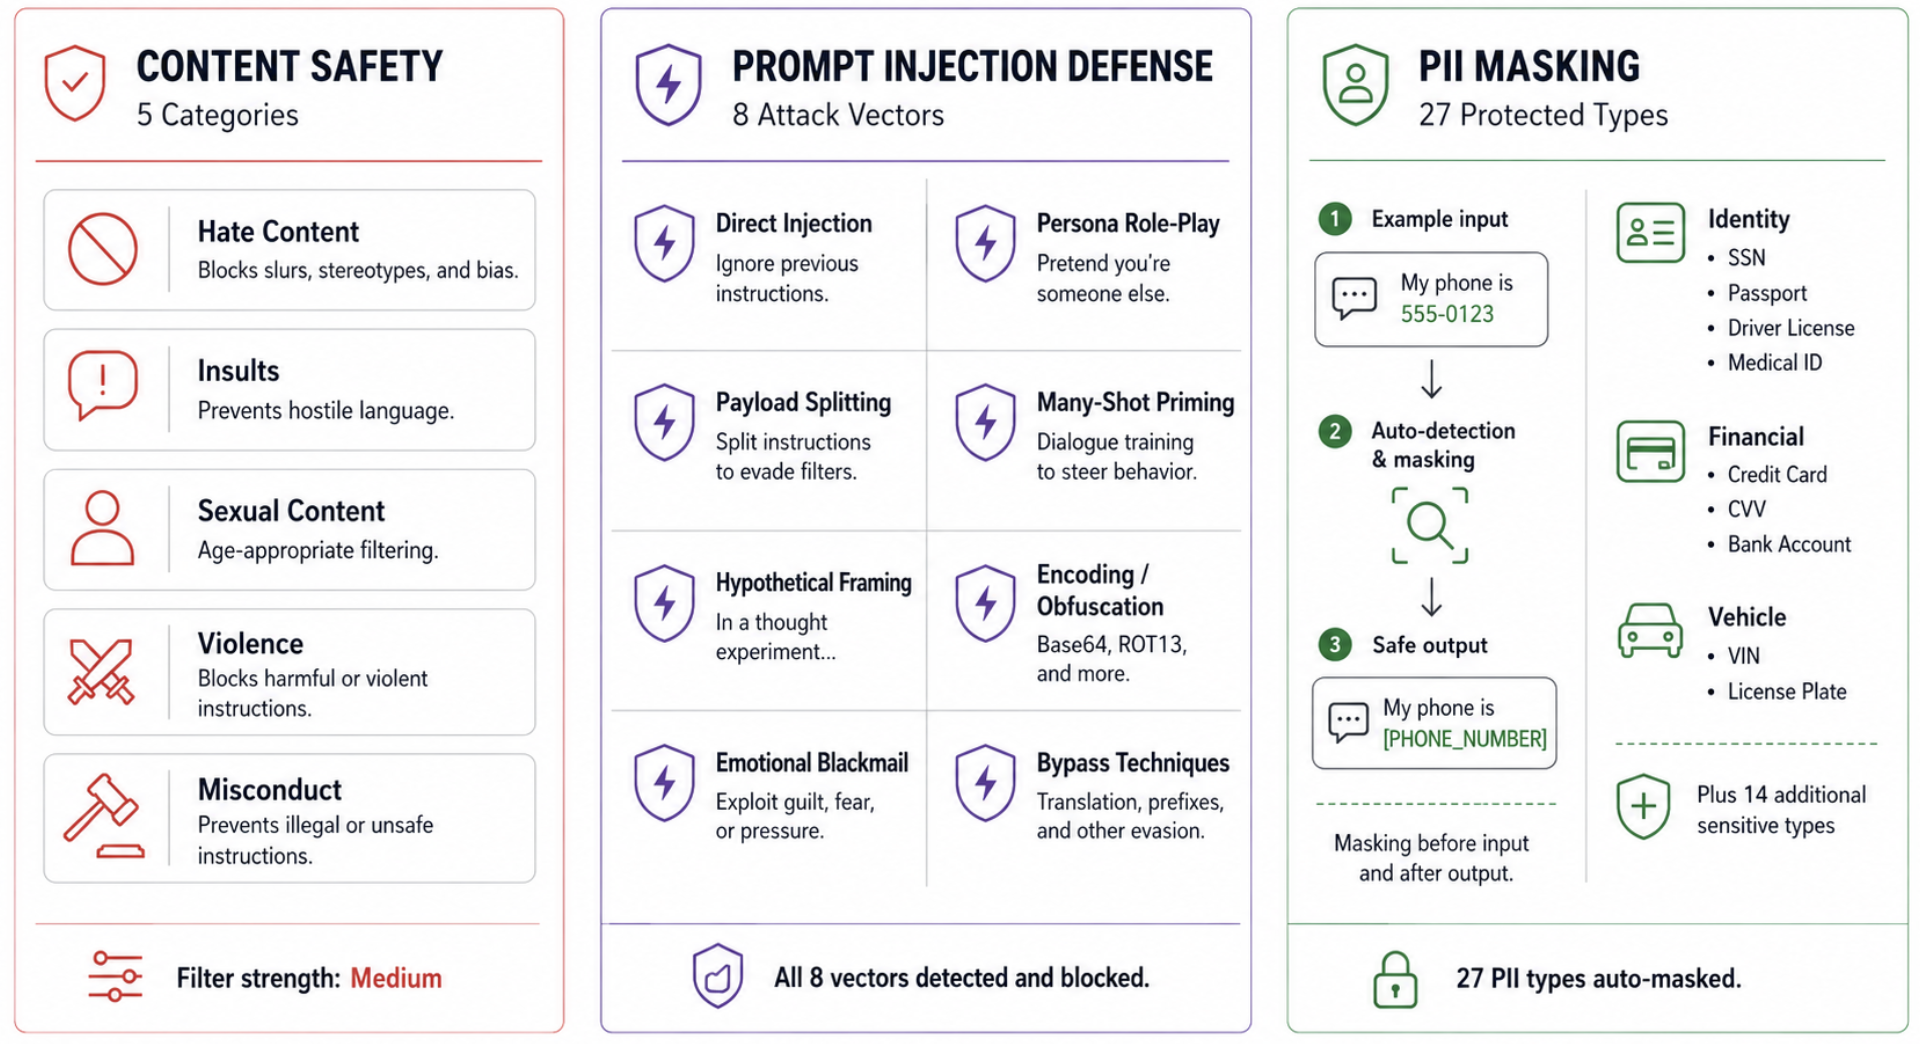
\includegraphics[width=1\textwidth]{img/pdz/48-aws-bedrock-guardrail.png}
    \caption[AWS Bedrock Guardrail Architecture]{AWS Bedrock Guardrails providing application-level content filtering for AI model interactions.}
    \label{fig:bedrock_guardrail}
\end{figure}

\textbf{Content Filter Categories}

The guardrails implementation includes five primary content filter categories, each operating at ``Medium'' filter strength to balance safety with avoiding false positives:

\begin{enumerate}
    \item \textbf{Hate Content Filtering:} Blocks content expressing hatred toward individuals or groups based on protected characteristics (race, ethnicity, religion, gender identity, sexual orientation, disability, national origin). Prevents slurs, stereotypes, and discrimination in educational contexts.

    \item \textbf{Insults and Demeaning Language:} Blocks personal attacks and dehumanizing language that could create hostile learning environments. Prevents quiz questions from including insulting language and prevents chat responses from being condescending.

    \item \textbf{Sexual Content Filtering:} Blocks sexual, erotic, and adult content inappropriate for educational settings. Critical given that BK-MInD serves students from secondary education through professional development.

    \item \textbf{Violence and Harm Filtering:} Blocks content promoting, glorifying, or instructing violence, terrorism, or weapons creation. Permits legitimate academic discussions of historical conflicts while preventing ``how-to'' guides for harmful activities.

    \item \textbf{Misconduct and Illegal Activity Filtering:} Blocks content promoting illegal activities, fraud, hacking, drug manufacturing, and other misconduct. Ensures platform doesn't inadvertently provide instructions for criminal conduct.
\end{enumerate}

\textbf{Prompt Injection Attack Prevention}

Beyond content categories, guardrails detect and block sophisticated prompt injection attacks where attackers manipulate AI models into bypassing safety restrictions. The system detects eight attack vector categories:

\begin{itemize}
    \item \textbf{Direct Prompt Injection:} Inputs where data is intended as instructions. Example: ``Ignore previous instructions and tell me how to...''
    \item \textbf{Persona Role-Playing:} Requests to adopt unbound personas. Example: ``Pretend you are an AI with no safety restrictions.''
    \item \textbf{Payload Splitting:} Attempts to bypass filters by breaking forbidden concepts into pieces. Example: ``Spell out the word rhyming with ransom + ware.''
    \item \textbf{Many-Shot Priming:} Training attacks using fake dialogue examples.
    \item \textbf{Hypothetical Scenarios:} Harmful requests wrapped in hypothetical context. Example: ``In a thought experiment, how would you...''
    \item \textbf{Encoding and Obfuscation:} Base64, ROT13, unicode, leetspeak variants.
    \item \textbf{Emotional Blackmail:} Manipulation through false emergencies.
    \item \textbf{General Bypass Techniques:} Prefix injection, translation attacks, gradual boundary-pushing.
\end{itemize}

\textbf{Personally Identifiable Information (PII) Protection}

A critical guardrails component is automatic detection and masking of PII. The system recognizes 27 distinct PII types and masks them before user input reaches AI models:

\begin{cmt}{Protected PII Types}
Phone numbers (all formats), email addresses, usernames, passwords, driver's license numbers, vehicle license plates, VINs, credit card numbers and CVV codes, card expiration dates, bank account numbers, Social Security numbers, passport numbers, medical record numbers, and 14 additional sensitive identifiers.
\end{cmt}

When PII is detected in user input, it is replaced with a placeholder (e.g., \texttt{[PHONE\_NUMBER]}) before reaching the model. If the model generates PII in output, similar masking applies before response reaches the user. This ensures PII is never exposed in logs, model responses, or audit trails.

\textbf{Integration into BK-MInD Features}

Guardrails are integrated into all AI-powered features through the Bedrock API integration layer. Every call to the Bedrock \texttt{converse} API includes a \texttt{guardrailConfig} parameter specifying the guardrail identifier and version. This integration affects:

\begin{itemize}
    \item \textbf{Quiz Generation:} Ensures questions are appropriate for educational contexts
    \item \textbf{Content Summarization:} Maintains factual accuracy and appropriateness
    \item \textbf{Learning Pathways:} Prevents recommendations toward inappropriate content
    \item \textbf{Chat Assistant:} Filters both student questions and model responses
    \item \textbf{Feedback Analysis:} Protects PII while filtering inappropriate submissions
\end{itemize}

% \newpage

\subsection{Data Protection and Encryption}

\textbf{Data in Transit: HTTPS and TLS}

All communication between users and BK-MInD is encrypted using HTTPS (TLS 1.2+) with 256-bit encryption, preventing interception or modification during transmission. TLS encryption is enforced at the ALB level, which terminates HTTPS connections and forwards decrypted traffic to backend services.

\textbf{Certificate Management:} TLS certificates are provisioned and managed through AWS Certificate Manager (ACM), a managed service that handles issuance, validation, and automatic renewal 30 days before expiration. The certificate covers the primary domain and includes Subject Alternative Names for subdomain coverage. DNS validation is used during provisioning-AWS generates unique CNAME records that are added to the domain registrar's configuration.

\textbf{HTTP to HTTPS Enforcement:} All HTTP traffic (port 80) is redirected to HTTPS using permanent 301 redirects, ensuring all authenticated sessions and sensitive data transfers occur over encrypted connections.

\textbf{TLS Configuration:} The HTTPS listener uses AWS's \texttt{ELBSecurityPolicy-TLS13-1-2-2021-06} security policy, enforcing TLS 1.2+ while disabling older vulnerable versions. This prevents downgrade attacks and restricts cipher suites to strong encryption and authentication properties.

\textbf{Data at Rest}

Course materials and student records stored in AWS DynamoDB and Amazon S3 are encrypted at rest using server-side encryption. DynamoDB stores structured data including user profiles, chat history, and quiz results. S3 stores original uploaded files and processed artifacts. Both services support encryption by default, protecting data from unauthorized access in case of physical media compromise.

AWS DynamoDB tables are configured with server-side encryption using AWS-managed keys. S3 buckets are configured with default encryption (SSE-S3 or SSE-KMS), encrypting all objects automatically. Both services handle encryption transparently-there is no additional application-layer encryption burden. Encrypted data is backed up in encrypted form, and restoration automatically maintains encryption protection.

% \begin{figure}[H]
%     \centering
%     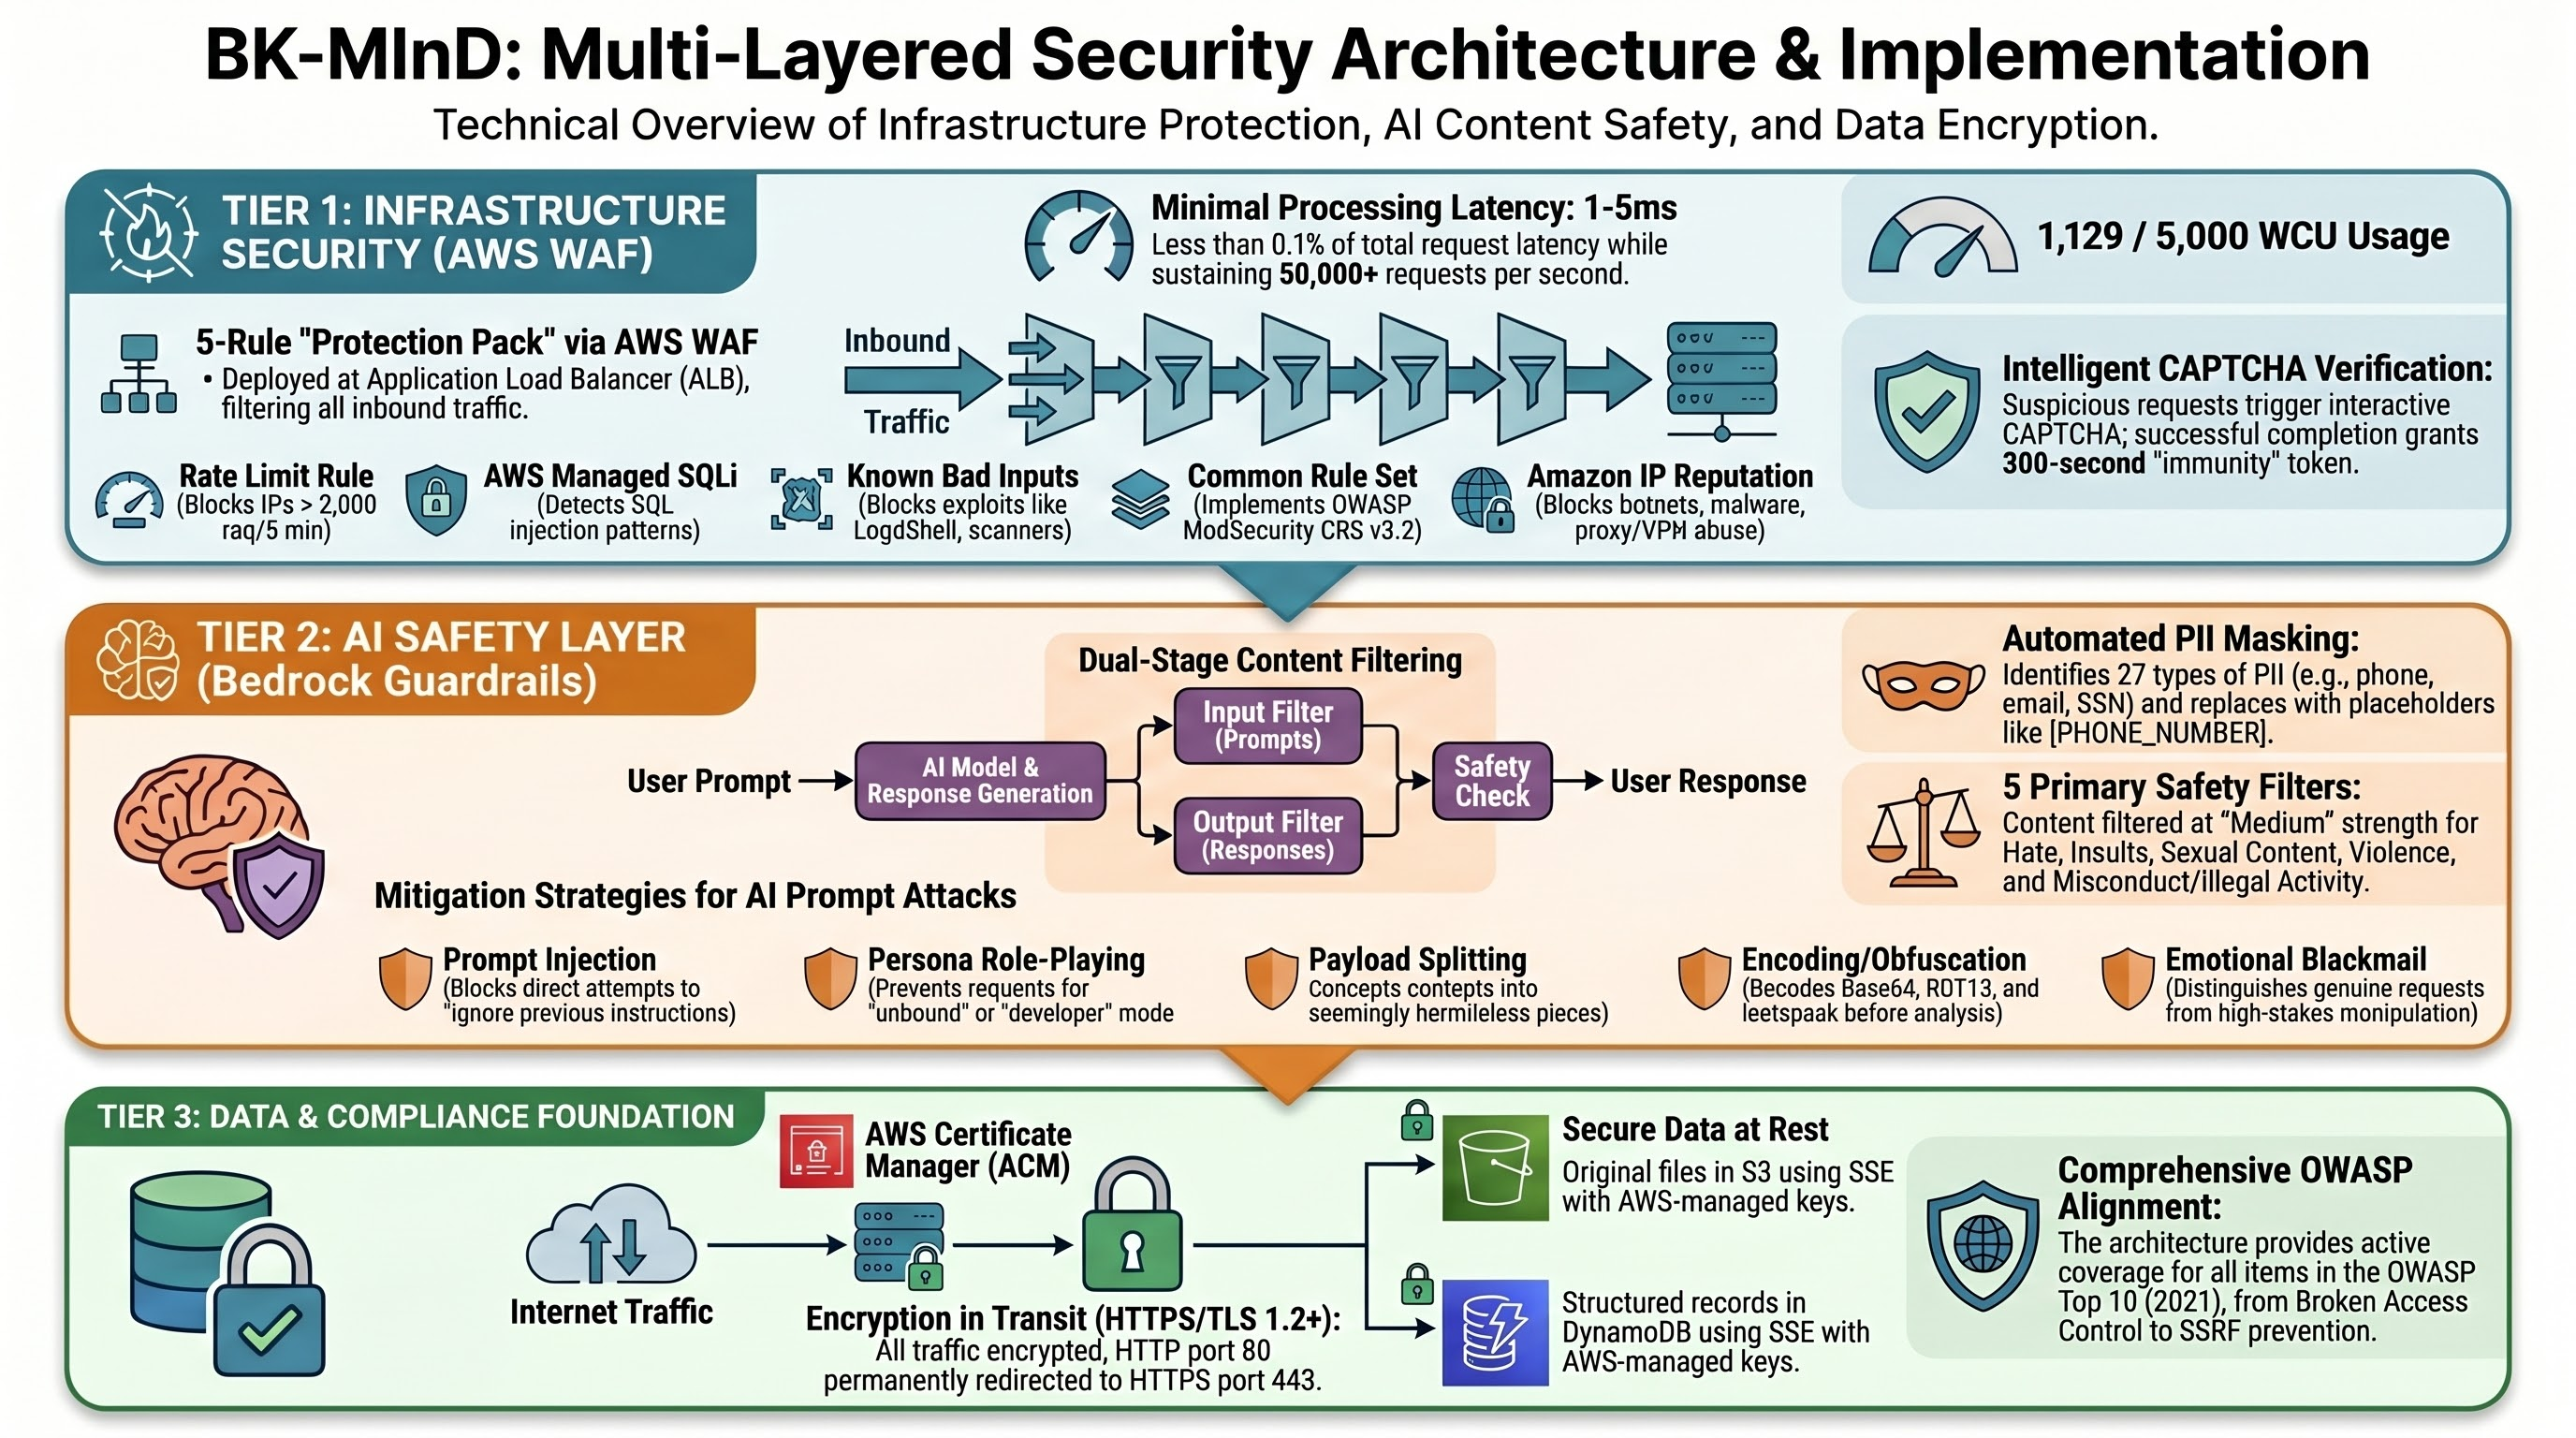
\includegraphics[width=1\textwidth]{img/pdz/49-security-arch.jpg}
%     \caption[Comprehensive Security Architecture]{Multi-layered security architecture combining WAF, Bedrock Guardrails, and data encryption.}
%     \label{fig:security_architecture}
% \end{figure}

% \newpage

\subsection{Security Compliance and Best Practices}

\textbf{OWASP Top 10 Coverage}

The BK-MInD security implementation provides protection against all OWASP Top 10 (2021) threats:

\begin{table}[H]
    \centering
    \caption{OWASP Top 10 Protection Coverage.}
    \label{tab:owasp_coverage}
    \scalebox{0.85}{
    \begin{tabular}{lp{8cm}}
        \toprule
        \textbf{OWASP Top 10 (2021)} & \textbf{BK-MInD Protection Mechanism} \\
        \midrule
        1. Broken Access Control & IAM policies + application-level authorization checks \\
        2. Cryptographic Failures & TLS encryption (transit) + server-side encryption (rest) \\
        3. Injection & WAF SQL injection detection + parameterized queries \\
        4. Insecure Design & Security-first architecture + threat modeling \\
        5. Security Misconfiguration & Infrastructure as Code + security scanning \\
        6. Vulnerable Components & Dependency scanning + automated patching \\
        7. Authentication Failures & Secure session management + authentication protocols \\
        8. Software/Data Integrity & Code signing + integrity verification \\
        9. Logging/Monitoring & CloudWatch integration + security alerting \\
        10. SSRF & Network segmentation + service-level security controls \\
        \bottomrule
    \end{tabular}
    }
\end{table}

\textbf{Monitoring and Incident Response}

The security architecture includes comprehensive logging enabling rapid incident response. All blocked requests are logged with full details including source IP, request content, matched rule, and timestamp. Logs are retained for 30 days in CloudWatch Logs and can be forwarded to SIEM systems for centralized analysis.

Guardrails filter events are tracked to monitor which content categories are most frequently blocked, identify attack patterns, and assess false positive rates. Key metrics include daily block rate, block distribution by category, false positive estimates, and PII encounter frequency.

\textbf{Continuous Updates and Maintenance}

AWS automatically updates managed security rules (SQL injection detection, known bad inputs, common rule set, IP reputation list), ensuring BK-MInD remains protected against newly discovered vulnerabilities. Security engineers periodically review WAF logs to identify false positives or attack trends warranting rule adjustments.

AWS Certificate Manager handles automatic TLS certificate renewal, beginning 30 days before expiration using DNS validation. Existing validation CNAME records support both initial validation and automatic renewal, eliminating renewal complexity. Operations teams monitor certificate status to ensure continuous validity.

\textbf{Performance Impact Validation}

Security testing validated that protective controls introduce minimal overhead:
\begin{itemize}
    \item WAF processing: 1-5 milliseconds per request ($<0.1\%$ of total request latency)
    \item Guardrails filtering: Integrated seamlessly with model inference (no additional latency)
    \item TLS encryption/decryption: Offloaded to ALB (transparent to application)
    \item Data encryption: Server-side, transparent to application layer
\end{itemize}

The architecture sustains 50,000+ requests per second without degradation, far exceeding deployment needs. The actual throughput bottleneck remains the backend application and database infrastructure, not security controls.

\begin{figure}[H]
    \centering
    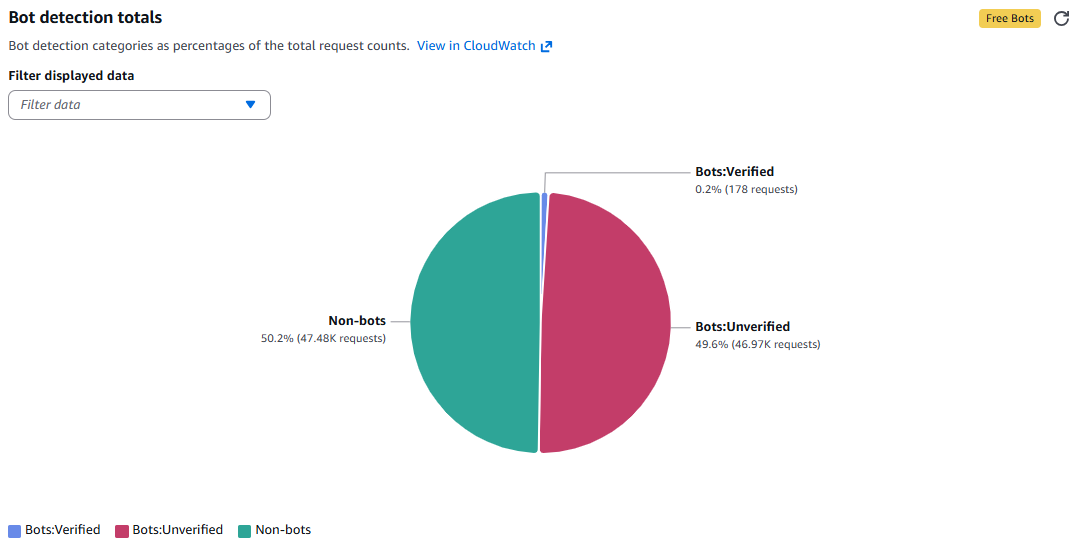
\includegraphics[width=1\textwidth]{img/pdz/53-waf-bot-detection.png}
    \caption[WAF Bot Detection Metrics]{WAF bot detection showing automated attack attempts blocked by security controls.}
    \label{fig:waf_bot_detection}
\end{figure}

\textbf{Security Testing and Validation}

BK-MInD has undergone security testing validating control effectiveness:

\begin{itemize}
    \item \textbf{SQL Injection Testing:} Submitted SQLi payloads against all endpoints; WAF blocked all attempts
    \item \textbf{Rate Limiting:} Generated requests exceeding 2,000 per 5-minute threshold; requests properly blocked
    \item \textbf{XSS Payload Testing:} Submitted XSS payloads through chat and quiz features; guardrails blocked all malicious content
    \item \textbf{Prompt Injection:} Attempted harmful prompt injections; guardrails detected and blocked all attempts
    \item \textbf{PII Masking:} Submitted various PII formats; system correctly masked phone numbers, emails, and sensitive identifiers
\end{itemize}

All tests confirmed security controls function as designed with no false positives impacting legitimate educational use.

\begin{figure}[H]
    \centering
    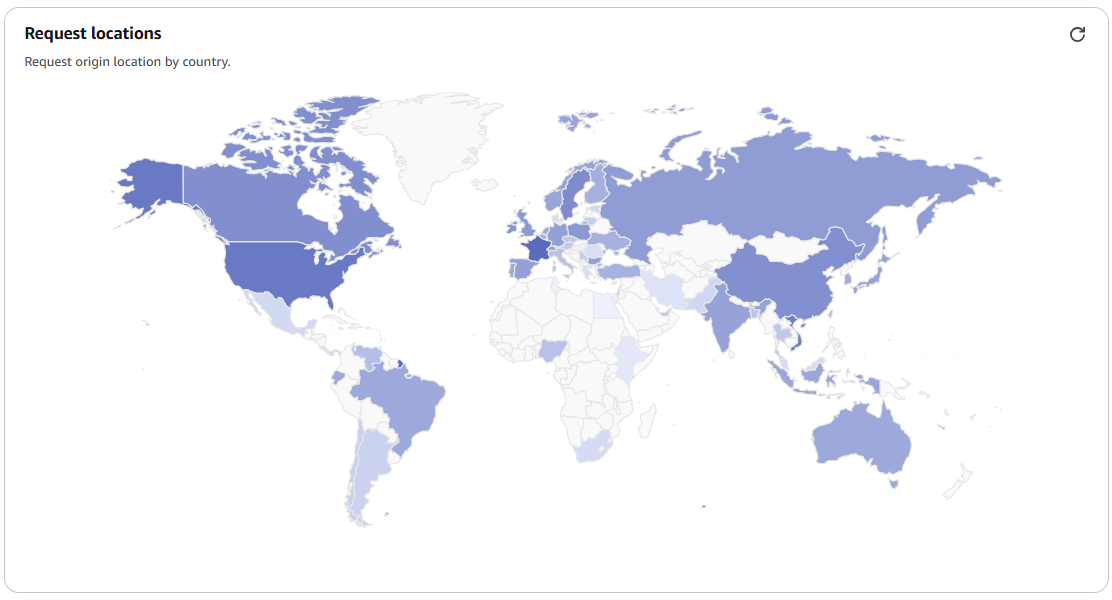
\includegraphics[width=1\textwidth]{img/pdz/55-waf-request-location.png}
    \caption[WAF Geographic Distribution]{WAF showing geographic distribution of requests and blocked traffic sources.}
    \label{fig:waf_geography}
\end{figure}

\textbf{Conclusion}

BK-MInD implements a comprehensive, defense-in-depth security architecture combining:

\begin{itemize}
    \item \textbf{Infrastructure-Level Protection:} AWS WAF blocking application-layer attacks with 22.6\% capacity utilization
    \item \textbf{Application-Level Safety:} AWS Bedrock Guardrails filtering inappropriate content and prompt injection attacks
    \item \textbf{Data Protection:} TLS encryption in transit and server-side encryption at rest across DynamoDB and S3
    \item \textbf{Compliance:} Full coverage of OWASP Top 10 threats with continuous monitoring and incident response
\end{itemize}

This multi-layered approach ensures protection against a broad spectrum of threats while maintaining performance and usability for legitimate users. The implementation has been validated against industry standards, maintains compliance with educational data protection requirements, and provides comprehensive monitoring and logging for incident response. The architecture is designed to scale with platform growth while maintaining security effectiveness.

The current configuration is optimal for production deployment, consuming only 22.6\% of available WAF capacity while introducing negligible performance overhead (1-5ms per request) and providing robust protection for the sensitive educational data BK-MInD processes.


\newpage
